\chapter{Unequal Mass Binary Neutron Star Simulations with M1 Neutrino Transport: Ejecta and Neutrino Emission}

\chaptermark{Unequal Mass BNS Simulations with M1}

\section{Chapter Overview}

\textit{The material in this chapter is based on ”Unequal Mass Binary Neutron Star Simulations with M1 Neutrino Transport: Ejecta and Neutrino Emission" by Trevor Vincent, Francois Foucart, Roland Haas, Matthew Duez, Lawrence Kidder, Harald Pfeiffer, Mark Scheel being prepared for Phys. Rev. D.}

%from sekiguchi
We present twelve new simulations of unequal mass neutron star mergers. The simulations were preformed with the SpEC code, and utilize nuclear-theory based equations of state and a two-moment gray neutrino transport scheme with an improved energy estimate based on evolving the number density. We model the neutron stars with the SFHo, LS220 and DD2 equations of state (EOS) and we study the neutrino and matter emission of all twelve models to search for robust trends between binary parameters and emission characteristics. We find that the total mass of the dynamical ejecta exceeds $0.01M_\odot$ only for SFHo with weak dependence on the mass-ratio across all models.  We find that the  ejecta have a broad $Y_e$ distribution ($\approx 0.06-0.48$), with mean $0.2$. $Y_e$ increases with neutrino irradiation over time, but decreases with increasing binary asymmetry. We also find that the models have ejecta with a broad asymptotic velocity distribution ($\approx 0.05-0.7c$). The average velocity lies in the range $0.2c - 0.3c$ and decreases with binary asymmetry. Furthermore, we find that disk mass increases with binary asymmetry and stiffness of the EOS. $Y_e$ of the disk increases with softness of the EOS. Finally, the strongest neutrino emission occurs for the models with soft EOS and we find no significant dependence of the magnitude or angular distribution of the neutrino luminosity with mass-ratio except in the case of the heavier (non-electron) neutrino species. %% \Francois{What do you mean by `morphology' here? Asymmetry should lead to more/less tidal tails, which I would as a different morphology - EDIT reading the manuscript, I know understand that it is the angular dependence of the neutrino luminosity. We should probably clarify}
\section{Introduction}

%% \Francois{In the text, I'd rather say $1.2M_\odot+1.44M_\odot$, or $q=1.2$, rather than 12144 which is hard to read}
%% \Francois{Update legend to use english rather that SpEC-language} \red{TV: ?}

%%%%%%%%%%%%%%%%%%%%%%%%%%%%%%%%%%%%%%%%%%%%%%%%%%%%%%%%%%%%%%%%%%%%%%%%%%%%%%%
The binary NS merger GW170817 was a landmark event, combining the first detection of gravitational waves
with an observation of a short gamma ray burst and a kilonova ~(\cite{theligoscientific:2017qsa,gbm:2017lvd,2017apj...848l..13a,ajello2018fermi}). Following the event, studies emerged analyzing many aspects of GW170817, from the
internal structure of neutron stars~(\cite{read:2008iy,delpozzo:13,lackey2014,gw170817-nsradius,gw170817-pe}), to the production of short gamma-ray bursts~(\cite{moch:93,lee1999a,janka1999,gbm:2017lvd,2017apj...848l..13a,2018natur.561..355m}) and the synthesis of r-process elements~(\cite{  li:1998bw,1976apj...210..549l,rosswog:1998hy, 2005astro.ph.10256k,2010mnras.406.2650m,metzger2017,2017sci...358.1559k,2017sci...358.1556c,2017apj...848l..19c,2017sci...358.1556c,cowperthwaite:2017dyu,2017natur.551...80k,2017sci...358.1583k,2017apj...848l..32m,2017apj...848l..18n,2017natur.551...67p,2017natur.551...75s,2017apj...848l..16s,2017apj...848l..27t,2017sci...358.1565e}). with the increasing sensitivity of advanced gravitational wave
interferometers many binary neutron star (BNS) detections will
be made in the next decade (\cite{ligo2018gwtc}).

Numerical simulations of mergers
play a crucial role in efforts to model the gravitational
wave signal, predict the properties of its electromagnetic counterparts,
and estimate the production of r-process elements from the merger. In this work, we
focus on the matter and neutrino emissions from BNS mergers. In particular we look at the ejecta
and neutrino emission from a new set of twelve asymmetric-mass ratio BNS simulations
which extends a previous set of 4 equal mass ratio BNS simulations (\cite{foucart:2015gaa}). While asymmetric-mass ratio
BNS simulations have been studied before in the context of general-relativistic-radiation
hydrodynamics, e.g. (\cite{sekiguchi2016dynamical}), (\cite{lehner2016unequal}), (\cite{radice2016dynamical}),
these previous studies use either a less advanced neutrino scheme and/or
different mass-ratios and EOS. Thus this paper adds to the ongoing effort to simulate
BNS systems and characterize their observables.

Neutrino interactions were first included in general relativistic simulations of neutron star mergers through a simple leakage scheme (\cite{sekiguchi:2011zd}), based on approximate methods developed for Newtonian simulations (\cite{ruffert1996,rosswog:2003rv}). A leakage scheme uses the local properties of the fluid and an estimate of the neutrino optical depth to determine the amount of energy lost locally to neutrino-matter interactions, and the associated change in the composition of the fluid. Leakage schemes provide an order-of-magnitude accurate estimate of neutrino cooling in the post-merger remnant, and have thus been used to capture the first-order effect of neutrino-matter interactions in general relativistic simulations of compact binary mergers (\cite{sekiguchi:2011zd,wanajo2014,lehner2016unequal,radice2016dynamical,palenzuela2015,deaton2013black,foucart2014neutron}). The inclusion of neutrino-matter effects with the leakage scheme, while crude, significantly affected the composition, morphology and total mass of the outflows, with some studies showing a factor 2 difference in total ejecta mass (\cite{radice2016dynamical}). However, most implementations of leakage do not account for irradiation of low density regions by neutrinos emitted from hot, dense regions. This potentially leads to large errors in the composition of the outflows, mostly by underestimating the number of protons (\cite{foucartm1:2016,foucart2015post}). Accordingly, the simplest leakage schemes are very inaccurate when attempting to predict the properties of post-merger electromagnetic signals. The only general relativistic simulations going beyond leakage use a moment formalism with an analytic closure to approximate the Boltzmann equation (\cite{1981mnras.194..439t,shibata:11}). In particular, neutron star merger simulations have been performed with a gray M1 scheme (\cite{foucartm1:2016,foucart2015post,sekiguchi2015dynamical,sekiguchi2016dynamical}), in which the energy density and flux density of each neutrino species are evolved. In BNS mergers, the use of this moment formalism showed that a range of compositions and thus of nucleosynthesis outcomes, exists in the material ejected by the merger (\cite{wanajo2014}). 

%% The gray M1 scheme is far from perfect. One obvious limitation is the impact of the analytical closure, which causes
%% unphysical shocks in regions where neutrinos converge.
%% This occurs in the polar regions of post-merger remnants,
%% putting into question the accuracy with which we can recover the composition of the polar outflows in those systems.
%% Another limitation is the lack of information about the energy spectrum of the neutrinos, or even their average energy. In (\cite{foucartm1:2016,foucart2015post}), for example, neutrinos in optically thick regions
%% are assumed to be in equilibrium with the fluid, which is reasonable, but neutrinos in optically thin regions are assumed
%% to follow everywhere a blackbody spectrum with a temperature determined from the average properties of the neutrino
%% radiation predicted by the simpler leakage scheme. This neglects potentially important spatial variations in the neutrino
%% spectrum, deviations from a blackbody spectrum, and the effects of relativistic beaming on the neutrino energies. These
%% approximations could easily affect our ability to predict the composition of the ejected material, as many neutrino-matter
%% cross-sections scale as the square of the neutrino energy. Additionally, the transport method used in (\cite{foucart:2015gaa}) does not guarantee conservation of the total lepton number. To handle this, in addition to the neutrino energy density and flux density, we now evolve the neutrino number density. This does not provide
%% us with any information about the shape of the neutrino spectrum, but does provide a local estimate of the average neutrino
%% energy, and accounts for relativistic beaming. By evolving the
%% neutrino number density, we can also guarantee conservation
%% of the total lepton number. \Francois{I wonder if this paragraph is too detailed for the intro, given that the evolution of $N$ is not a major point of our study.}

Previous studies of asymmetric mass-ratio BNS systems with fully general-relativistic radiation-hydrodynamics include
(\cite{sekiguchi2016dynamical,lehner2016unequal,radice2018binary}). Sekiguchi et al.~(\cite{sekiguchi2016dynamical}) studied two EOS, SFHo and DD2 with mass ratios between .86 and 1.0 and a fixed total mass of $2.7M_\odot$ to around 30-ms post-merger using a M1 neutrino transport scheme. They found that for SFHo the ejecta mass depended weakly on mass-ratio, but the average electron number per baryon decreased with mass ratio. For DD2 these trends were reversed. They also found that only the soft EOS, SFHo, produced ejecta mass above $0.01M_\odot$. Lehner et al.~(\cite{lehner2016unequal}) studied three EOS, NL3, SFHo and DD2 with mass ratios between .76 and 1.0 and a fixed total mass of $2.7M_\odot$ at 3-ms post-merger using a neutrino leakage scheme. They found that there was a greater ejecta mass with increasing binary asymmetry. Unlike Sekiguchi et al., Lehner et. al found that none of the EOS produced ejecta above $0.01M_\odot$. Finally, Radice et al. (\cite{radice2018binary}) studied four EOS, BHB$\Lambda\phi$, SFHO, DD2 and LS220, with mass ratios between .85 and 1.0 and a fixed total mass of $2.7M_\odot$ to around 20-ms post-merger  using a neutrino leakage scheme and a viscous hydrodynamics scheme. Radice et al./ found that  none of their models produced ejecta over $0.01M_\odot$ and their numbers agreed with Lehner et al.~(\cite{lehner2016unequal}). The discrepancy between these results could however be due different choices for the definition of the unbound material in these studies. This paper adds onto previous works in the following ways. First, we look at a different set of parameters not found in the above studies. We use the SFHo, LS220 and DD2 EOS to study the effects of EOS on the merger emissions. We use mass-ratios ranging from $q \sim.76-1$ to study the effects of mass asymmetry on emissions. Unlike the previous studies, we do not fix the total mass and allow it to vary from $\sim 2.5-2.9M_\odot$. On top of this, we use a new M1 neutrino transport scheme which evolves the number density, allowing for consistent lepton number evolution (\cite{foucart:2016rxm}). 

We organize the paper as follows. In Section~\ref{sec:num_imp}, we discuss the numerical implementation we use and the
equations we solve, including the gray-M1 scheme for neutrino transport. In the following
sections of the paper, we discuss the matter and neutrino emission from a new set of
twelve binary neutron star merger simulations, ranging in mass ratio and equation of state.
Finally we conclude with ideas for future work. We use a system of units such
that $c = G = M_\odot = 1$, where c is the speed of light in
vacuum, G is the gravitational constant, and $M_\odot$ is the mass
of the Sun. We use Einstein's convention of summation over
repeated indices. Latin indices run over 1, 2, 3, while Greek
indices run over 0, 1, 2, 3. The spacetime metric signature is $(-,+,+,+)$.

%% During inspiral, our standard resolution for the fluid
%% grid covering the neutron star has grid spacing ∆x ≈
%% 200m. During merger, the fluid grid allows up to 7 nested
%% layers of grid boxes; ∆x doubles with each layer outward.
%% The innermost box – centered on the black hole – covers
%% a half-width of around 40 km with ∆x ≈ 240m. Our
%% previous study [14] reports convergence tests for BHNS
%% binaries using the DD2 EOS and resolutions similar to
%% ours. We have also simulated the plunge and early merger
%% phase (about 4 ms) of two cases in the current study at
%% 20% lower resolution: FSU with a 1.4  star and SFHo
%% with a 1.2  star. We find that post-merger mass predictions
%% agree to 10% for unbound matter and to 1% for
%% total baryonic mass outside the black hole (with more
%% ejecta at higher resolution), while the ejecta average velocity
%% and black hole irreducible mass track each other
%% almost identically. Assuming second order convergence,
%% this would correspond to 20% and 2% errors in ejecta
%% and disk mass, respectively. This would be in addition to
%% any errors related to initial data and inspiral, the former
%% being difficult to assess because our usual eccentricity reduction
%% procedure was not very effective for the small
%% initial binary separations used in this study. Resolutions
%% of the sort used here are needed to track the thin stream
%% of matter that flows to the black hole when the neutron
%% star tidally disrupts. If a segment of this stream is less
%% than about 10 points across, unphysical heating, shocks,
%% and mass ejection can result. We check for the absence of
%% such sy


\section{Numerical Implementation}
\label{sec:num_imp}
\subsection{General Overview}
%% We evolve using the SpEC code. Details of SpEC’s
%% methodology for non-vacuum systems can be found in
%% our earlier papers [14, 30]. To summarize, the spacetime
%% is evolved pseudospectrally on one grid, while the fluid is evolved using conservative shock-capturing techniques on another grid.
%% Neutrino effects are treated using a 3-flavor energy-integrated
%% neutrino leakage scheme, which can capture
%% effects on the fluid of emitting neutrinos but not of absorbing
%% them.


We evolve Einstein's equations and the general relativistic equations of ideal radiation-hydrodynamics using the Spectral Einstein Code (SpEC)(\cite{specwebsite}). SpEC evolves those equations on
two separate grids: a pseudospectral grid for Einstein's equations, written in the generalized harmonic formulation (\cite{lindblom2006}),
and a finite volume grid for the general relativistic equations
of neutrino-hydrodynamics, written in conservative form. The latter
makes use of an approximate Riemann solver (HLL (\cite{hll}))
and high-order shock capturing methods (fifth order WENO
scheme (\cite{liu1994200,jiang1996202})), resulting in a second-order accurate evolution scheme. For the time evolution, we use a third-order
Runge-Kutta algorithm. Finally, after each time step, the two
grids communicate the required source terms, using a third-order accurate spatial interpolation scheme. Those source terms are the metric and its derivatives (from the pseudospectral grid to the finite volume grid) and the fluid variables, which are rest-mass density, pressure, spatial velocity, the Lorentz factor and enthalpy. The following sections will give more detail on individual segments of this numerical method.

In the following sections, we make use the 3+1 decomposition of the metric
%
\begin{align}
  ds^2 &= g_{\alpha\beta}dx^\alpha dx^\beta \\
  &= -\alpha^2dt^2 + \gamma_{ij}(dx^i + \beta^i)(dx^j + \beta^j)
\end{align}
%
where $\alpha$ is the lapse, $\beta^i$ the shift, and $\gamma_{ij}$ the 3-metric on a slice of constant coordinate t. The extension of $\gamma_{ij}$ to the full 4-dimensional space is the projection operator:
%
\begin{equation}
  \gamma_{\alpha\beta} = g_{\alpha\beta} + n_\alpha n_\beta.
\end{equation}
%

%% In our current scheme, the radiation stress-energy
%% tensor does not self-consistently feed back onto the evolution
%% of Einstein’s equations. Direct measurements of the energy
%% in the neutrino sector shows that the radiation energy density
%% is everywhere negligible as far as gravitational interactions
%% are concerned. The neutrino stress-energy tensor is, however,
%% fully coupled to the general relativistic equations of hydrody-
%% namics. More details about these numerical methods can be
%% found in (Reference here).

%% We run Gr-hydro with M1 as described.
%% Grid Setup
%% Atmosphere choices
%% Reconstruction choices
%% what is turned on and off code
%% Tracers

\subsection{Initial Data}

Initial data for this simulation was produced by an BNS initial data solver based on the work of Foucart~{\it et
al}. for BHNS systems (\cite{foucart2008initial}), which was built upon the elliptic solver Spells (\cite{pfeiffer2003}) and further improved for BNS systems in (\cite{tacik2015binary}) and (\cite{haas:2016}). We start by considering systems in quasi-equilibrium, where time
derivatives vanish in a corotating frame. We take the metric to be conformally flat and solve for the lapse,
shift, and conformal factor using the extended conformal thin sandwich (XCTS) equations (\cite{pfeiffer2003b}). The matter in the stars is modeled as a cold perfect fluid with an irrotational velocity profile.

Low eccentricity can be achieved through an iterative procedure requiring the evolution of the system for 2-3 orbits in each iteration (\cite{pfeiffer2007reducing}). All of the simulations in this paper use that algorithm to achieve estimated eccentricities of approximately $e\sim 0.001$.

Neutrinos are initialized in thermal equilibrium with the fluid. For more details see (\cite{foucart2016impact}).

%% \Francois{Neutrinos are initialized in thermal equilibrium with the fluid, i.e. basically to zero energy density as the initial star is cold. You can refer to the M1 code paper for details.}

\subsection{Spacetime Evolution}

%% \matt{Is there anything new here?  Should we just refer to earlier papers, or are we aiming to make this paper self-contained?}

%% We evolve Einstein's equations and the general relativistic equations of ideal hydrodynamics using the SpECTRAL Einstein Code (SpEC). SpEC evolves those equations on two separate grids: a pseudospectral grid for Einstein's equations, written in the generalized harmonic formulation and a finite volume grid for the general relativistic equations of hydrodynamics, written in conservative form. The latter makes use of an approximate Riemann solver (HLL) and high-order shock capturing methods (fith order WENO), resulting in a second order accurate evolution scheme. For the time evolution, we use a third-order Runge-Kutta algorithm. Finally after each time step, the two grids communicate the required source terms, using a third order accurate spatial interpolation scheme. Those source terms are the metric and it's derivatives (from the pseudospectral grid to the finite volumegrid) and the stress-energy tensor of the fluid (from the finite volume grid to the pseudospectral grid). In our current scheme, the radiation energy density is everywhere negligible as far as gravitational interactions are concerned. More details about these numerical methods can be found in.
%
The Einstein field equations can be written in the form
%
\begin{equation}
  \label{eqn:efe}
R_{\alpha\beta} = 8\pi\left(T_{\alpha\beta} - \frac{1}{2}\psi_{\alpha\beta}T\right),
\end{equation}
%
where $R_{\alpha\beta}$ is the Ricci tensor, $\psi_{\alpha\beta}$ is the metric tensor and $T_{\alpha\beta}$ is the stress energy tensor with trace T. SpEC uses the generalized harmonic decomposition (\cite{lindblom2006}) to write the Einstein field equations in a form that allows stable numerical computation.

In the generalized harmonic formalism, the evolution of the coordinates follows the wave equation
%
\begin{equation}
  \label{eqn:gh_coordinates}
  \psi_{ab}\nabla^c\nabla_cx^b = H_a\left(x^e\right),
\end{equation}
%
where $\psi_{ab}$ is the spacetime metric, and $H_a(x^c)$ a set of four arbitrary functions. Using Eq.~(\ref{eqn:gh_coordinates}) we can rewrite 
Eq.~(\ref{eqn:efe}) as (\cite{pretorius2005numerical})
%
\begin{equation}
  \begin{split}
  \label{eqn:efe_gh}
  \psi^{\delta\gamma}\partial_\gamma\partial_\delta\psi_{\alpha\beta} + \partial_\beta\psi^{\gamma\delta}\partial_\gamma\psi_{\alpha\delta} &+ \partial_\alpha\psi^{\gamma\delta}\partial_\gamma\psi_{\beta\delta} + 2\partial_{(\beta,} H_{\alpha)} \\
  - 2H_\delta\Gamma^\delta_{\alpha\beta} + 2\Gamma^\gamma_{\delta\beta}\Gamma^{\delta}_{\gamma\alpha} &= -8\pi(2T_{\alpha\beta} - g_{\alpha\beta}T),
  \end{split}
\end{equation}
%
where the Christoffel symbols $\Gamma^\delta_{\alpha\beta}$ are defined by
%
\begin{equation}
\Gamma^\gamma_{\alpha\beta} = \frac{1}{2}\psi^{\gamma\epsilon}\left(\partial_\beta\psi_{\alpha\epsilon} + \partial_\alpha\psi_{\beta\epsilon} \partial_\epsilon\psi_{\alpha\beta}\right).
\end{equation}
%
Eq.~(\ref{eqn:efe_gh}) introduces four independent gauge functions $H_\alpha$, which need to be chosen. Before the merger of the neutron stars, we set
%
\begin{equation}
H_\alpha\left(x^i_c,t\right) = H_\alpha\left(x^i_c,0\right)\exp\left(-\frac{t^2}{\tau^2}\right),
\end{equation}
%
with $\tau = \sqrt{d^3_0/M}$, $d_0$ the initial separation, M is the total mass of the binary at infinite separation and $x^i_c$ are comoving spatial coordinates which follow the rotation and inspiral of the binary. The initial data is constructed in a gauge $H^{initial}_a$ that assumes the time derivatives in the comoving frame are zero. At the beginning of the simulation, we set $H_a\left(x^i_c,0\right) = \Hat H_a$, where $\Hat H_a$ is a tensor that agrees with $H^{initial}_a$ in a frame comoving with the grid and is constant in time. The gauge will thus evolve into the harmonic condition $H_a = 0$. During merger, we find that transitioning to the ``damped harmonic'' gauge condition is better (\cite{szilagyi2014key}). Defining
%
\begin{equation}
  H_\alpha = \left(\log{\frac{\sqrt{\gamma}}{\alpha}}\right)^2\left(\frac{\sqrt{\gamma}}{\alpha}t_\alpha - \gamma_{\alpha i} \frac{\beta^i}{\alpha}\right),
\end{equation}
%
we transition according to
%
\begin{equation}
  H_\alpha(t) = H_\alpha\left(1-\exp{\frac{-(t-t_{DH})^2}{\tau_{m}^2}}\right),
\end{equation}
%
with $t_{DH}$ the time at which we turn on the damped harmonic gauge and $\tau_m = 100M$.

With these gauge choices we solve a first order representation of the generalized harmonic system (Eq.~\ref{eqn:efe_gh}) in which the fundamental variables are the spacetime metric $\psi_{ab}$, its spatial first derivatives $\phi_{iab}$ and its first derivatives in the direction normal to the $t=$constant slice $\Pi_{ab}$. The generalized harmonic first order system is then:

\begin{align}
  \partial_t\psi_{ab} &- (1 + \gamma_1)N^k\partial_k\psi_{ab} = -N\Pi_{ab} - \gamma_1N^i\Phi_{iab},  \\
  \partial_t\Pi_{ab} &- N^k\partial_k\Pi_{ab} + Ng^{ki}\partial_k\Phi_{iab} - \gamma_1\gamma_2N^k\partial_k\psi_{ab} \\
  &= 2N\psi^{cd}(g^{ij}\Phi_{ica}\Phi_{jdb} - \Pi_{ca}\Pi_{db} - \psi^{ef}\Gamma_{ace}\Gamma_{bdf}) \notag\\
  &-2N\nabla_{(a}H_{b)} - \frac{1}{2}Nt^ct^d\Pi_{cd}\Pi_{ab} - Nt^c\Pi_{ci}g^{ij}\Phi_{jab} \notag\\
  &+N\gamma_0[2\delta^c_{(a}t_{b)} - \psi_{ab}t^c](H_c + \Gamma_c) - \gamma_1\gamma_2N^i\Phi_{iab}\notag\\
    &-2\alpha(T_{ab} - \frac{1}{2}\psi_{ab}T^{cd}\psi_{cd}),\notag \\
  \partial_t\phi_{iab} &- N^k\partial_k\phi_{iab} + N\partial_i\Pi_{ab} - \gamma_2N\partial_i\psi_{ab} \\
  & = \frac{1}{2}Nt^ct^d\Phi_{icd}\Pi_{ab} + Ng^{jk}t^c\Phi_{ijc}\Phi_{kab} - N\gamma_2\Phi_{iab}\notag,
\end{align}
%
where
%
\begin{align}
  &\partial_t\psi_{ab} := - N\Pi_{ab} + N^i\phi_{iab}, \\
  &\partial_i\psi_{ab} := \phi_{iab}.
\end{align}
%
This amounts to a symmetric hyperbolic system of 50 coupled nonlinear equations. The constraint damping parameters $\{\gamma_0,\gamma_1,\gamma_2\}$ are additional free parameters which dampen any constraint violating modes which may grow due to small numerical errors in the evolution. To set the $\gamma$ parameters we use a trial-and-error process which concludes when we find that the constraint-violating modes do not grow significantly over time. In practice, we set the parameters to
%
\begin{align}
\gamma_1 &= 0.999 (f(r_c, 10d) - 1), \\
\gamma_2 &= \frac{.005}{M}+\frac{3}{M_1}f(r^i_1, 2.5R_1)\notag\\
&+\frac{3}{M_2}f(r^i_2, 2.5R_2)+\frac{.075}{M_2}f(r^i_c, 2.5d), \\
\gamma_2 &= \frac{.005}{M}+\frac{.2}{M_1}f(r^i_1, 2.5R_1)\notag\\
&+\frac{.2}{M_2}f(r^i_2, 2.5R_2)+\frac{.075}{M_2}f(r^i_c, 2.5d), \\
f(r^i&,w) = \exp(-|r^i|^2/w^2),
\end{align}
%%
where $r^i_{1,2,c}$ correspond to the coordinate locations of the first neutron star, second neutron star and center of mass respectively, $R_1/M_1$ is the radius and mass of the 1st neutron star, $R_2/M_2$ is the radius and mass of the 2nd neutron star, $M = M_1 + M_2$ and $d$ is the separation of the two neutron star centers.

\subsection{Neutrino Evolution}

We use a gray two moment M1 scheme for neutrino transport introduced in (\cite{foucart2016impact}). To recap, the new scheme has the advantages of exactly conserving the total lepton number, and taking into account spatial variations in the neutrino energy. In this section we will give an overview of the scheme we use.

For each neutrino $\nu_i$ we can describe the neutrinos by their distribution function $f_{\nu}(x^\mu, p^\mu)$ where $x^\mu = (t, x^i)$ gives the time and the position of the neutrinos and $p^\alpha$ is the 4-momentum of the neutrinos. The distribution function $f_{(\nu)}$ evolves according to the Boltzmann equation:
%%
\begin{equation}
  p^\alpha\left[ \frac{\partial f_{(\nu)}}{\partial x^\alpha} - \Gamma^\beta_{\alpha\gamma}\frac{\partial f_{(\nu)}}{\partial p^\beta}\right] = \left[\frac{df_{(\nu)}}{d\tau}\right].
\end{equation}

In general, this is a 7-dimensional problem which is extremely expensive to solve numerically. Approximations to the Boltzmann equation have thus been developed for numerical applications. In this work, we consider the moment formalism developed by Thorne (\cite{1981mnras.194..439t}) and Shibata et al.~(\cite{shibata:11}), in which only the lowest moments of the distribution function in momentum space are evolved.  We limit ourselves to the use of this formalism in the gray approximation, that is we only consider energy-integrated moments.  We will consider three independent neutrino species: the electron neutrino $\nu_e$, the electron antineutrinos $\bar \nu_e$, and the heavy lepton neutrinos $\nu_X$. The latter represents the 4 species $(\nu_\mu, \bar \nu_\mu, \nu_\tau, \bar \nu_\tau)$. This merging is justified because the temperatures and neutrino energies reached in our merger calculations are low enough to suppress the formation of the corresponding heavy leptons. The presence of heavy leptons would then require including the charged current neutrino interactions that differentiate between these individual species.

In the gray approximation with the first two moments of the distribution function, we evolve for each species projections of the stress-energy tensor of the neutrino radiation $T^{\mu\nu}_{rad}$. We write

\begin{equation}
T^{\mu\nu}_{rad}  = Ju^\mu u^\nu + H^\mu u^\nu + H^\nu u^\mu + S^{\mu\nu},
\end{equation}
%
with $H^\mu u_\mu = S^{\mu\nu}u_\mu = 0$ and $u^\mu$ the 4-velocity of the fluid. We can decompose the momentum as follows

\begin{equation}
  p^\alpha = \nu(u^\alpha + l^\alpha),
\end{equation}

with $l^\alpha u_\alpha = 0$ and $l^\alpha l_\alpha = 1$. With this decomposition, the energy $J$, flux $H^\mu$ and stress tensor $S^{\mu\nu}$ of the neutrino radiation as observed by an observer comoving with the fluid are related to the neutrino distribution function by

\begin{align}
  J &= \int^\infty_0 \mathrm{d}\nu \nu^3 \int \mathrm{d}\Omega f_{(\nu)}(x^{\alpha}, \nu, \Omega) \\
  H^\mu &= \int^\infty_0 \mathrm{d}\nu \nu^3 \int \mathrm{d}\Omega f_{(\nu)}(x^{\alpha}, \nu, \Omega) l^{\mu}\\
  S^{\mu\nu} &= \int^\infty_0 \mathrm{d}\nu \nu^3 \int \mathrm{d}\Omega f_{(\nu)}(x^{\alpha}, \nu, \Omega) l^{\mu}l^\nu,
\end{align}
%
where $\nu$ is the neutrino energy in the fluid frame, $\int\mathrm{d}\Omega$ denotes integrals over solid angle on a unit sphere in momentum space, and
%
%
We also utilize the decomposition of $T^{\mu\nu}_{rad}$ in terms of the energy, flux and stress tensor observed by an inertial observer,

\begin{equation}
  T^{\mu\nu}_{rad} = En^\mu n^\nu + F^\mu n^\nu + F^\nu n^\mu + P^{\mu\nu},
\end{equation}
%
with $F^\mu n_\nu = P^{\mu\nu}n_\mu = F^t = P^{t\nu} = 0$, and $n^\alpha$ the unit normal to a $t$ = constant slice.

We define a projection operator on the reference frame of an observer comoving with the fluid:
%
\begin{equation}
  h_{\alpha\beta} = g_{\alpha\beta} + u_\alpha u_\beta.
\end{equation}
%
We can then write equations relating the fluid frame variables to the inertial frame variables

\begin{align}
  E &= W^2 J + 2 W v_\mu H^\mu + v_\mu v_\nu S^{\mu\nu}, \\
  F_\mu &= W^2 v_\mu J + W(g_{\mu\nu} - n_\mu v_\nu) H^\nu \\
  &+ W v_\mu v_\nu H^\nu + (g_{\mu\nu} - n_\mu v_\nu) H^\nu + Wv_\mu v_\nu H^\nu \notag\\
  &+ (g_{\mu\nu} + n_\mu v_\nu) v_\rho S^{\nu\rho}, \notag\\
  P_{\mu\nu} &= W^2 v_\mu v_\nu J + W(g_{\mu\nu} - n_\mu v_\rho)v_\nu H^\rho \\
  &+ (g_{\mu\rho} - n_\mu v_\rho)(g_{\nu\kappa} - n_\nu v_\kappa)S^{\rho\kappa} \notag \\
  &+ W(g_{\rho\nu} - n_\rho v_\nu) v_\mu H^\rho \notag
\end{align}

using the decomposition of the 4-velocity
%
\begin{equation}
  \label{eqn:vel_decomp}
  u^\mu = W(n^\mu + v^\mu),
\end{equation}
%
where $v^\mu n_\mu = 0$ and $W = \sqrt{1 + v_i v^i}$.

By taking moments of the Boltzmann equation, the evolution equations for $\tilde E = \sqrt{\gamma}E$ and $\tilde F = \sqrt{\gamma} F^i$ can then be written in conservative form

\begin{align}
  \partial_t \tilde E &+ \partial_j (\alpha \tilde F^j - \beta^j \tilde E) \\
  &= \alpha(\tilde P^{ij} K_{ij} - \tilde F^j \partial_j \ln \alpha - \tilde S_\text{rad}^\alpha n_\alpha), \notag\\
  \partial_t \tilde F_i &+ \partial_j (\alpha \tilde P_i^j - \beta^j \tilde F_i) \\
  &= (-\tilde{E} \partial_i \alpha + \tilde{F}_k \partial_i \beta^k + \frac{\alpha}{2} \tilde{P}^{jk} \partial_i \gamma_{jk} + \alpha \tilde{S}_{\text{rad}}^\alpha \gamma_{i\alpha}) \notag,
\end{align}
%
where $\gamma$ is the determinant of $\gamma_{ij}$, $\tilde{P}_{ij} = \sqrt{\gamma}P_{ij}$, and $\tilde{S}_{rad}^\alpha = \sqrt{\gamma} S_{rad}^\alpha$ includes all collisional source terms. Additionally, we consider the number current density for each species of neutrino:

\begin{equation}
  N^\mu = Nn^\mu + \mathcal{F}^\mu,
\end{equation}
%
where N is the number density of neutrinos, and $\mathcal{F}^\mu$ the number flux density. We can define the average neutrino energy in the fluid frame by

\begin{equation}
  N^\mu = \frac{Ju^\mu + H^\mu}{\langle \nu \rangle}, 
\end{equation}
%
which then gives us an estimate for the energy

\begin{equation}
\langle \nu \rangle = W\frac{(E-F_iv^i)}{N},
\end{equation}
%
where $W$ is the Lorentz factor introduced in Eq.~\ref{eqn:vel_decomp}. The evolution equation for $\tilde{N} := \sqrt{\gamma}N$ is

\begin{equation}
  \partial_t \tilde N + \partial_j(\alpha \sqrt{\gamma} \mathcal{F}^j - \beta^j \tilde N) = \alpha \sqrt{\gamma} C_{(0)}.
\end{equation}

To close this system of equations we need three additional ingredients: a prescription for the computation of $P^{ij}(E, F_i)$ which is called the closure relation, a prescription for the computation of the number flux $\mathcal{F}^j$ (specific to te evolution of the number density N in this paper) and the collisional source terms $\tilde{S}^\alpha, C_{(0)}$.

For $P^{ij}(E, F_i)$  we use the M1 approach and interpolate between optically thick and thin limits:

\begin{equation}
P^{ij} = \frac{3p-1}{2}P^{ij}_{\text{thin}} + \frac{3(1-p)}{2}P^{ij}_{\text{thick}}.
\end{equation}

Here the parameter p is known as the variable Eddington factor and the functional form of p in terms of the lower moments $H,J$ is known as the M1 closure. Our choices for $P^{ij}_{\rm thin}, P^{ij}_{\rm thick}$ and $p$ are discussed in the Appendix of (\cite{foucartm1:2015}).

For $\mathcal{F}^i$, by definition we have

\begin{equation}
  \mathcal{F}^i = \frac{JWv^i}{\langle \nu \rangle} + \frac{\gamma^i_\mu H^\mu}{\langle \nu^F \rangle}
\end{equation}
%
where the flux-weighted average neutrino energy,  $\langle \nu^F \rangle$ is computed in such a way to take the effects of a finite optical depth on the spectrum into account, see (\cite{foucart:2015gaa}) for details.

For the source terms $\tilde{S}^\alpha$, we assume the fluid has an energy-integrated emissitivity $\bar \eta$ due to the charged-current reactions
%
\begin{align}
  p + e^- &\rightarrow n + \nu_e, \\
  n + e^+ &\rightarrow p + \bar{\nu}_e,
\end{align}
%
as well as electron-positron pair annihilation
%
\begin{equation}
  e^+ + e^- \rightarrow \nu_i \bar \nu_i,
\end{equation}
%
plasmon decay
%
\begin{equation}
  \gamma \rightarrow \nu_i\bar \nu_i,
\end{equation}
%
and nucleon-nucleon Bremsstrahlung
%
\begin{equation}
  N + N \rightarrow N + N + \nu_i + \bar \nu_i.
\end{equation}
%
The inverse reactions are responsible for an energy-averaged absorption opacity $\bar \kappa_a$. We also consider an energy-averaged scattering opacity $\bar \kappa_s$ due to elastic scattering of neutrinos on nucleons and heavy nuclei. Neglecting other reactions (e.g. inelastic scatterings and $\nu\bar\nu$ annihilation) the source terms $S^\alpha$ can then be shown to be (\cite{shibata2011truncated})
%
\begin{equation}
  \tilde S_\text{rad}^\alpha = \sqrt{\gamma} [\bar \eta u^\alpha - \bar \kappa_\alpha J u^\alpha - (\bar \kappa_a + \bar \kappa_s) H^\alpha].
\end{equation}
%
The collisional source term for the number density $\bar N$ is given by
%
\begin{equation}
  C_{(0)} = \bar \eta_N - \bar \kappa_N \frac{J}{\langle\nu\rangle} = \bar \eta_N - \frac{\bar \kappa_N J \bar N}{W(\bar E - \bar F_iv^i)}.
\end{equation}
%
Thus we need the energy integrated emissivities $(\bar \eta, \bar \eta_N)$ and the energy-averaged opacities $(\bar \kappa_A, \bar \kappa_S, \bar \kappa_N)$ to compute the source terms. To do this we need the equilibrium energy-integrated emissivities $(\bar \eta^{eq}, \bar \eta^{eq}_N)$ and equilibrium opacities $(\bar \kappa^{eq}_A, \bar \kappa^{eq}_S)$ which assume a Fermi-Dirac distribution with temperature $T_{\rm fluid}$. When they are available, we use the equilibrium emissitivies and opacities from Ruffert et al.~(\cite{ruffert1996}), except for nucleon-nucleon Bremsstrahlung for which the emissivity is computed following Burrows et al.~(\cite{burrows2006b}). When either an equilibrium emissitivity or opacity is not available for a reaction, we compute whichever is unknown using Kirchoff's Law:

\begin{equation}
\bar \eta^{eq} = \bar\kappa^{eq}\int B_{(\nu)}\mathrm{d}\nu,
\end{equation}

where $B_{(\nu)}$ is the blackbody spectrum in equilibrium with the fluid. See (\cite{foucart2016impact}) for more details.
%% \Francois{I think that we take the emissivities and $\kappa_s^{eq}$ from these references, but set $\kappa_a^{eq}$ using Kirkhoff's law ($\eta^{eq}/\kappa_a^{eq}=B$, with $B$ the energy density for black-body radiation in equilibirum with the fluid). For some reactions, we do the opposite (set $\eta^{eq}$ from $\kappa_a^{eq}$ and Kirkhoff's law). The details are in the M1 code paper.}
After computing the equilibrium quantities, we make the choices
%
\begin{align}
  \bar \eta &= \bar \eta^{eq}, \\
  \bar \eta_N &= \bar \eta_N^{eq}, \\
  \bar \kappa_A &= \bar \kappa^{eq}_A\frac{T_\nu^2}{T_{\text{fluid}}^2}, \\
  \bar \kappa_S &= \bar \kappa^{eq}_S\frac{T_\nu^2}{T_{\text{fluid}}^2},
\end{align}
%
where $T_\nu$ is the neutrino temperature computed from the neutrino energy and number density, assuming a blackbody spectrum (see (\cite{foucart2016impact}) for more details). Lastly we set
%
\begin{equation}
\bar \kappa_N = \bar \kappa_A \frac{\bar\eta_N}{\bar\eta}\frac{F_3(\eta_\nu)T_{fluid}}{F_2(\eta_\nu)},
\end{equation}
%
where $\eta_\nu = \mu_\nu/T$ with $\mu_\nu$ the chemical potential of neutrinos in equilibrium with the fluid and $F_k(\eta_\nu)$ the Fermi integral:
%
\begin{equation}
F_k(\eta_\nu) = \int^\infty_0\frac{x^k}{1 + \exp(x - \eta_\nu)}\mathrm{d}x.
\end{equation}
%
%% with $\bar \eta_N$ the energy-integrated number emission and $\bar \kappa_N$ the energy-averaged number absorption.  We first compute the
%% eqenergy-averaged absorption κ̄ of charge-current processes, Athe energy-integrated emissivity η̄ eq of thermal processes, and eq
%% the energy-averaged scattering opacities κ̄ for neutrinos in Sequilibrium with the fluid. We use the emissivities and opaci-
%% ties proposed by Ruffert et al. [78] for all reactions, except for nucleon-nucleon Bremsstrahlung for which the emissivity is
%% computed following Burrows et al. [79]. We can then compute the equilibrium absorption opacities of charged current reac-
%% tions and emissivities of thermal processes using Kirchoff’s law.



%% \begin{equation}
%%   \bar \eta^{eq} = \bar \kappa^{eq} \int B_{(\nu)}(T, \mu_\nu)mathrm{d}\nu
%% \end{equation}

\subsection{Fluid Evolution}

The neutron stars are described by ideal fluids with stress tensor
%%
\begin{equation}
T_{\mu\nu} = \rho_0 h u_\mu u_\nu + Pg_{\mu\nu},
\end{equation}
%
where $\rho_0$ is the rest mass density, h the specific enthalpy, P the pressure and $u^\mu$ the 4-velocity. The general relativistic equations of hydrodynamics are evolved in conservative form, using the conservative variables
%
\begin{align}
  %% \rho_* &= \rho_0W\sqrt{\gamma}, \\ %-\sqrt{\gamma}n_\mu u^mu /rho_0 \\
  \rho_* &= -\sqrt{\gamma}n_\mu u^\mu \rho_0, \\
  %% \tau &= \rho_* (hW - 1) - \sqrt{\gamma}P, \\ %\sqrt{\gamma}n_\mu n_\nu T^{\mu\nu} - \rho_* \\
  \tau &= \sqrt{\gamma}n_\mu n_\nu T^{\mu\nu} - \rho_*, \\
  %% S_k &= \rho_* h u_i, %-\sqrt{\gamma}n_\mu T^\mu_k
  S_k &= -\sqrt{\gamma}n_\mu T^\mu_k.
\end{align}
%
The 3 + 1 stress-energy conservation equations for radiation-hydrodynamics $\nabla_\nu T^{\mu\nu} = -S^\mu_\text{rad}$ and the baryon conservation equations $\nabla_\mu (\rho_0 u^\mu) = 0$ become (\cite{shibata2011truncated})
%
% From arxiv:1502.04146v1 FrancoisNSBHNeutrinoTransport2015
% From arXiv:1607.07450v2 FrancoisImprovedNeutrinEonergyEstimate 
% arxiv 1212.4810
% duez2008evolving
% Francois Thesis
%
\begin{align}
  \partial_t \rho_* + \partial_j(\rho_* v^j) =&\:0, \\
  \partial_t \tau + \partial_i (\alpha^2 \sqrt{\gamma} T^{0i} - \rho_* v^i) =& -\alpha \sqrt{\gamma} T^{\mu\nu} \nabla_\nu n_\mu\\
  &+ \alpha \tilde S_\text{rad}^\alpha n_\alpha, \notag\\
  \partial_t S_i + \partial_j(\alpha\sqrt{\gamma}T^j_i) =&\: \frac{1}{2}\alpha \sqrt{\gamma} T^{\mu\nu} \partial_i \gamma_{\mu\nu} \\
  &- \alpha \tilde S_\text{rad}^\alpha \gamma_{i\alpha}.\notag
\end{align}

\subsection{Composition Evolution}

The fluid composition in our simulations is described by the electron fraction:

\begin{equation}
  Y_e = \frac{n_p}{n_p + n_n},
\end{equation}

where $n_p$ and $n_n$ are the proton and neutron number densities, respectively (the net electron number density $n_{e^{-}} - n_{e^{+}} = n_p$, due to charge neutrality in the fluid). From lepton number conservation, we have:
%% \Francois{I'm not sure the implicit sum over species on the rhs is really standard Einstein's notation here}
%% \sout{From the conservation of electron fraction (\cite{shibata:11}):}
%% \Francois{There is no conservation of electron fraction - this is just the evolution of $Y_e$ in conservative form. I'd skip this and directly use the next equation, justified from lepton number conservation}
%% \begin{equation}
%%  \nabla_\mu (\rho Y_e) = \rho Q_e,
%% \end{equation}
%% \sout{where $Q_e$ is the electron generation rate and by lepton number conservation, we have}
%% $C_0$ by the electron capture and neutrino capture by nucleons or nuclei. Since $C_0$ is the change in the number density of neutrinos, while (rho*Q_e) is the change in (rho*Ye) = m_p * (change in number density of protons), and the change in the number of protons is also the change in the number of electrons. The link between C_0 and Q_e is then given by lepton number conservation, i.e. number of electrons - number of positrons + number of electron neutrinos - number of electron antineutrinos = constant
%% [and positrons don't survive long enough to be taken into account here]:

\begin{equation}
  \partial_t \left(\rho_* Y_e \right) + \partial_i\left(\rho_*Y_e v^i\right)= -\sum_{\nu}\textrm{sign}(\nu)\alpha \sqrt{\gamma} C^{\nu}_{(0)},
\end{equation}

where $\sum_{\nu}$ sums over neutrino species with $\textrm{sign}(\nu)$ set to 1 for $\nu_e$, -1 for $\bar \nu_e$, and 0 for $\nu_x$. Importantly for the electron fraction, evolving the neutrino number density $N$ frees us from having to guess at the average neutrino energy when computing the coupling to the fluid. It also guarantees that the source term for the evolution of the electron fraction of the fluid is fully consistent with the evolution of the neutrino number density, thus conserving the total lepton number of the system (\cite{foucart2016impact}). 
%% \Francois{Add citation to the first paper evolving $\tilde N$. Also, $\bar N \rightarrow \tilde N$}

\subsection{Equation of State (EOS)}

We use three finite-temperature, composition dependent nuclear-theory based equations of state. Two of them are based on relativistic mean field models (\cite{walecka1974theory}) and one based on the single nucleus approximation for heavy nuclei (\cite{lattimer1991generalized}). They are:

\begin{enumerate}
\item{DD2 (\cite{hempel:2011mk}): This EOS is based on nuclear statistical equilibrium with a finite volume correction coupled to a relativistic mean field theory for treating high-density nuclear matter. DD2 contains neutrons, protons, light nuclei such as deuterons, helions, tritons and alpha particles and heavy nuclei. DD2 does not satisfy the so-called flow-constraint (\cite{hempel2017well}).}
\item{
LS220 (\cite{lattimer1991generalized}): is based on the single nucleus approximation
for heavy nuclei where the thermal distribution of different nuclear species is replaced by a single representative heavy nucleus. LS220 contains  neutrons, protons, alpha particles and heavy nuclei. LS220 does not satisfy the constraints from Chiral effective field theory (\cite{hempel2017well}).
}
\item{SFHo (\cite{2013apj...765l...5s}): This EOS, like DD2, also uses an RMF model, containing neutrons, protons, light nuclei such as deuterons, helions, tritons and alpha particles and heavy nuclei. However, SFHo uses a different RMF parameterization,
specifically designed to match neutron star properties as inferred by observations. SFHo shows some minor
deviations from Chiral effective field theory calculations (\cite{hempel2017well}).
}
\end{enumerate}

\begin{figure}[H]
  \centering
  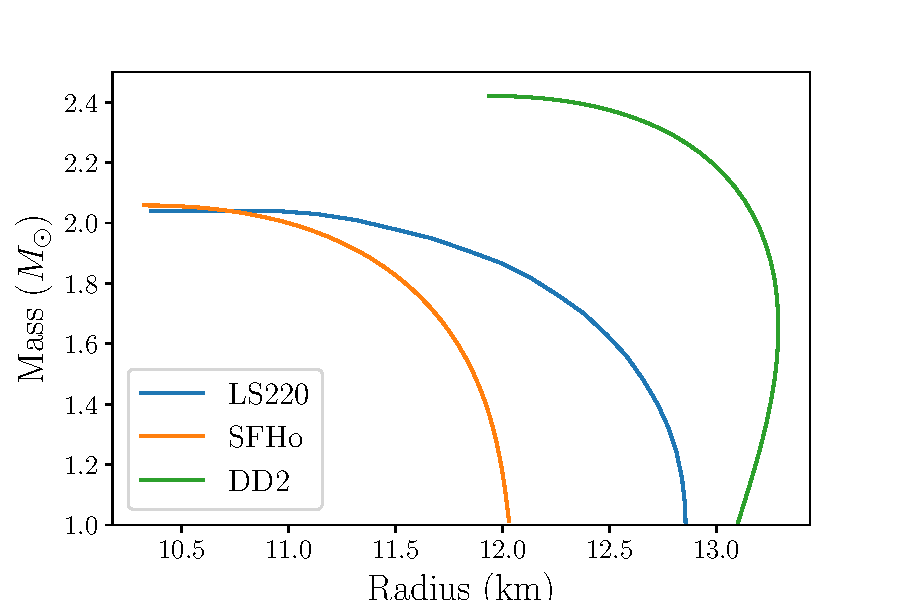
\includegraphics[width=.75\textwidth]{chap3/Figures/eos.png}
%% \begin{figure}[!htbp] \includegraphics[width=\textwidth]{chap3/Figures/dd2_ye_table.png}
\caption{
  M-R curves for each of the equations of states used in this work.
}
\label{fig:eos_mr}
\end{figure}

While each EOS shows deviations from theoretical calculations, they all have a radius, maximum mass and tidal deformalibity that are compatible with observations (\cite{demorest:2010bx,hempel2017well}). For all three equations of state, we show mass-radius curves in Figure~\ref{fig:eos_mr}. These curves were computed by integrating the TOV equations for the EOS by using the table values at $T=0.1$\,MeV in beta equilibrium. From Figure~\ref{fig:eos_mr}, we can clearly see that for each EOS there is a maximum mass for the non-rotating isolated neutron star. Furthermore we can associate with each EOS an average density at this maximum mass as $\langle \rho \rangle := 3M_{max}/4\pi R^3_{max}$ and the ratio of this average density and the central density $\rho_c$ of the star is an indication of how ``stiff'' the EOS is. Higher values of $\langle \rho \rangle/\rho_c$ correspond to stiffer EOS, while lower values correspond to softer EOS (\cite{bauswein2013prompt}). In our case, from stiffest to softest, the EOS are ranked DD2, LS220 and SFHo. Softer EOS tend to make smaller stars at a fixed mass. For a fiducial mass of $1.4M_\odot$, the radii are 13.2 km, 12.7 km, 11.9 km for DD2, LS220 and SFHo respectively. We can also introduce a useful quantity called the compactness, which is defined by $C=M/R$. Softer EOS tend to make more compact stars. The maximum mass however is not a good indicator of whether the post-merger remnant will promptly collapse to a black hole (BH) after merger because the remnant will most likely be differentially rotating and held up by centrifugal and thermal forces against collapse.
A more accurate estimate for the maximum mass at which the merger promptly collapses to a BH is given by Bauswein~{\it et al.}~(\cite{bauswein2013prompt}) who ran simulations of BNS mergers with a smoothed particle hydrodynamics code that employs the conformal flatness approximation of the Einstein field equations and includes a GW backreaction scheme to determine a thershold mass for prompt collapse across 12 different realistic EOS. Bauswein et al./ found the threshold masses for SFHo, LS220 and DD2 were $2.95M_\odot$, $3.05M_\odot$ and $3.35M_\odot$ respectively. Thus the SFHo and LS220 models are more likely to undergo prompt collapse for the higher end of the total masses considered in this paper ($\sim 2.9M_\odot$, see Sec.~\ref{sec:initial_models}). 

%% \begin{figure*}
%%   \includegraphics[width=\textwidth]{chap3/Figures/12132-ENua.png}
%% \label{fig:nulum_table_eos_12132}
%% \caption{
%%   Neutrino luminosity for 12132 runs at 10ms.
%% }
%% \end{figure*}

%% On the other hand, the DD2 EoS
%% uses the density-dependent relativistic mean-field (RMF)
%% interactions of Typel et al. (2010). Hempel et al. (2015) have
%% found a good agreement of cluster formation with nuclear
%% experiments in the DD2 EoS, but the NS radius with DD2 EoS
%% is inconsistent with the observations by (Steiner et al. 2013).
%% The SFHo EoS has similar nuclear properties to the DD2 EoS,
%% but the mass–radius is tuned to fit the NS radius observation
%% (Steiner et al. 2013).

%% M-vs-R curves for these EOS (evaluated at low temperature
%% and neutrinoless beta-equilibrium Ye) are plotted
%% in Fig.~\ref{fig:eos_all}.

%% \begin{figure}
%% \includegraphics[width=0.45\textwidth]{chap3/Figures/eos_all.png}
%% \label{fig:eos_all}
%% \caption{M-R curves for each of the EOSs for a cold neutron star in beta equilibrium.}
%% \end{figure}

%%  The maximum baryon mass of a cold, uniformly rotating neutron star
%% (as determined from mass-shedding sequences generated by
%% the code of Cook, Shapiro, and Teukolsky (\cite{cook94a,cook94b,cook94c})) is $2.83M_\odot$ for the LS220 equation of state, $2.86M_\odot$
%% for the SFHo equation of state, and $3.45M_\odot$ for the DD2 equation of state.



%% Hence, for the LS220 and SFHo equations of state, we expect \red{at higher binary masses,} a short-lived NS remnant which then collapses to a BH for most mass-ratios and total-masses in the observable range. 
%% \Francois{If the NS mass distribution peaks in the $(1.2-1.4)M)_\odot$ range, maybe all of them lead to uniformly rotating stars? Maybe we should also discuss the threshold mass for rapid collapse to a BH, from Bauswein et al. 2013.}However, for the DD2 EOS we expect a long-lived NS remnant.

\subsection{Initial Models}
\label{sec:initial_models}
We extend our previous work (\cite{foucart:2015gaa}) and study the merger
of unequal mass neutron star binaries with the neutrino M1 transport scheme introduced in (\cite{foucart2016impact}) and discussed above. We study mass ratios between .76 and 1 and masses between 1.2$M_\odot$ and 1.56$M_\odot$ which are both within the ranges of current binary neutron star observations (see e.g. (\cite{lattimer:2012nd})). We focus here on the late stages of the coalescence, comprising the last $3-5$ orbits (depending on EoS) before merger and we stop evolving any systems once they collapse. The parameters for the initial models and the type of post-merger remnants they create (before or as of 7.5-ms post-merger) are shown in Table \ref{tab:initial_models}. The specific grid setup for each model will be discussed in the following section.

\begin{table}
\centering
\begin{tabular}{cccccccccl} \toprule
Model & EOS & \(M_{1}\) & \(M_{2}\) & \(q\) & $C_1$ & $C_2$ & $d_0 (km)$  & Collapse?\\ \midrule
D144144 & DD2 & 1.44 & 1.44 & 1.0 & .161 & .161 & 48.7 & No \\
D12132 & DD2 & 1.2 & 1.32 & .91 & .134 & .147 & 48.7 & No\\
D12144 & DD2 & 1.2 & 1.44 & .83 & .134 & .161 & 48.7 & No\\
D12156 & DD2 & 1.2 & 1.56 & .77 & .134 & .173 & 48.7 & No\\
 \midrule
L144144 & LS220 & 1.44 & 1.44 & 1.0 &.175  &.175 & 44.3 & $(\sim 2 ms)$\\
L12132 & LS220 & 1.2 & 1.32 & .91 & .146 & .161  & 44.3 & No \\
L12144 & LS220 & 1.2 & 1.44 & .83 & .146  &.175  & 44.1 & No\\
L12156 & LS220 & 1.2 & 1.56 & .77 & .146  & .191 & 44.3 & $(\sim 4.5 ms)$\\
 \midrule
S144144 & SFHO & 1.44 & 1.44 & 1.0 &.179  & .179 & 44.3 & $(\sim .5 ms)$\\
S12132 & SFHO & 1.2 & 1.32 & .91 & .148  & .163  & 44.3 & No\\
S12144 & SFHO & 1.2 & 1.44 & .83 & .148  & .179 & 44.3 & No\\
S12156 & SFHO & 1.2 & 1.56 & .77 & .148  & .195 & 44.3 & $(\sim 1.4 ms)$\\
 \bottomrule
\end{tabular}
\caption{Parameters for the initial models presented in this paper. $M_1$ and $M_2$ are the gravitational masses of the two neutron stars, $C_1$ and $C_2$ are the compactness of the respective neutron stars and $d_0$ is the initial coordinate distance between the centers of stars. The last column gives the post-merger remnant as of 7.5-ms post-merger. If the binary collapsed before 7.5-ms a rough estimate for the time of collapse is shown in brackets.}
%% \Francois{Define all these quantities}}
\label{tab:initial_models}
\end{table}

%% DD2 12132, 12144, 12156, 144144
%% $ID_d = 32.8545;
%% $ID_d = 32.8493;
%% $ID_d = 32.8567;
%% $ID_d = 32.89;
%% LS220 12132, 12144, 12156, 144144
%% $ID_d = 29.8929;
%% $ID_d = 29.8425;
%% $ID_d = 29.8656;
%% $ID_d = 29.9043;
%% SFHO 12132, 12144, 12156, 144144
%% $ID_d = 29.9172;
%% $ID_d = 29.917;
%% $ID_d = 29.9071;
%% $ID_d = 29.9277;

\subsection{Grid Setup}

Before the two neutron stars enter into contact, the pseudospectral grid on which we evolve Einstein's equations takes advantage of the approximate spherical symmetry of the neighborhood of each star, and in the far-field region. The evolved spatial slice is decomposed into two small balls around the center of each neutron star, sets of spherical shells around each star, and distorted cubes to connect the three spherically symmetric regions. The inner ball is expanded into Zernike polynomials, the shells into Chebyshev polynomials (in radius) and spherical harmonics (in angle) and the distorted cubes in Chebyshev polynomials. The grid follows the centers of the neutron stars defined as the center of mass of the matter in the $x < 0$ and $x > 0$ half planes, through a simple rotation and scaling of the grid coordinates. We do not exploit the reflection symmetry $z \rightarrow -z$ in our runs.

We maintain this grid decomposition for the evolution of Einstein's equations up to the point at which the maximum density on the grid increases beyond the low-level oscillations observed during the inspiral. This rise in the density signifies the transition from two well-separated neutron star cores to a single, more massive object. At that point we switch to a grid which is fully centered on the coordinate center of mass of the system. This grid  is made of a ball at the origin of the coordinate system, surrounded by 59 spherical shells extending to the outer edge of the computational domain. Both before and after merger, the outer boundary is located at $40d_0$, with $d_0$ the initial separation of the binary, provided in Table~\ref{tab:initial_models}.

The finite volume grid on which we evolve the general relativistic equations of hydrodynamics is very simple. Before the two neutron stars get into contact, it is composed of two cubes, each centered on a neutron star and composed of $96^3$ cells.  In the coordinate system comoving with the neutron star centers, the neutron stars expand as the binary inspirals. To avoid losing matter to the outer boundary of the finite volume grid, we expand the grid by $4.5\%$ every time the flux of matter across the outer boundary exceeds $0.015 M_\odot s^{-1}$. As the inspiral lasts less than 10 ms, this implies a mass loss well below $10^{-4} M_\odot$ before merger. As the two neutron stars approach each other, the two finite volume boxes will eventually intersect. During merger, we would like to follow the forming massive neutron star remnant, the tidal tails, the accretion disk, and any ejected material. We switch to a finite difference grid centered on the forming remnant with 3 levels of refinement. Each level has, at our standard resolution $200^2 \times 100$ cells, with the finest grid spacing listed in Table~\ref{tab:grid_setup} and each coarser level increasing the grid spacing by a factor of 2. The lower number of cells in the vertical direction reflects the fact that the remnant is less extended in that direction, and thus that we do not need the finest grid to extend as far vertically as horizontally.

%% \Francois{Check that this matches your actual grid setup} During merger, we no longer assume equatorial symmetry.
%% This numerical resolution, although insufficient to capture the evolution of magnetic fields, has been shown to be provide reasonable accuracy in purely hydrodynamic simulations.
%% \Francois{We might want to be more precise, and provide references, if we make this claim.}

\begin{table}
\centering
\begin{tabular}{ccc}\toprule
Name & $\mathrm{d}x_{\text{ins}}$ (m) & $\mathrm{d}x_{\text{mer}}$ (m) \\ \midrule
D12132 & 279 & 300 \\
D12144 & 280 & 300 \\
D12156 & 279 & 300 \\
D144144 & 273 & 300 \\ \midrule
S12132 & 251 & 300 \\
S12144 & 250 & 300 \\
S12156 & 238 & 300 \\
S144144 & 238 & 300 \\ \midrule
L12132 & 252 & 300 \\
L12144 & 253 & 300 \\
L12156 & 252 & 300 \\
L144144 & 245 & 300 \\ \bottomrule
\end{tabular}
\caption{Finite difference grid sizes for the initial models. All simulations were set so that they would have a 300m resolution during merger. For reference, the DD2 $1.44M_\odot$ star has a $\sim 10.48 km$ radius in our grid coordinates.
 %% \Francois{Maybe compare to the size of neutron stars on the grid [It's a little disingenuous for us to compare grid size to NS sizes on your mass-radius plot, because stars are smaller in our grid coordinates (isotropic coordinates)].}
}
\label{tab:grid_setup}
\end{table}

\subsection{Ejecta Analysis}

In a BNS merger, matter expelled at high velocity may
ultimately become unbound from the central gravitational potential. Two indicators have been used to label matter unbound:
%
\begin{enumerate}
\item{$\mathbf{u_t < -1}$: For a stationary spacetime, $u_t$ (the projection of the 4-velocity along the timelike Killing vector field) is a constant of motion for geodesics. Assuming the space is also asymptotically flat, the Lorentz factor $W$ satisfies $W = -u_t$ at infinity. Therefore we may flag matter as unbound using the condition  $u_t < -1$.} \\
\item{$\mathbf{hu_t < -1}$: For a stationary relativistic fluid flow, the relativistic Bernoulli equation (\cite{rezzolla2013relativistic}) implies $hu_t$ is constant along fluid worldlines. In an asymptotically flat spacetime, we would expect $W = -u_t$ (if the fluid particles follow geodesics). Since the relativistic enthalpy $h$ is only defined up to a constant factor which can be set such that $h \leftarrow 1$ at spatial infinity. Therefore, we may flag matter as unbound using the condition $hu_t < -1$.
  %% \Francois{For tabulated equations of state, we do not have $h=1$ at $\rho=0$, due to nuclear binding energy. This can make it difficult to asses whether material with $-1.003<hu_t\lesssim -0.997$ is bound or unbound. We can talk about this more, but basically the only way to fix this is to account for out-of-nuclear-statistical-equilibrium evolution of the fluid, which we can't do at the moment.}
}
%% \red{TV: Okay this needs to be discussed sometime in a meeting then}
\end{enumerate}

We have found previously (\cite{foucart:2015gaa}) that the second indicator $hu_t < -1$, the Bernoulli criterion, produces
qualitatively more accurate results in SpEC, therefore all material labelled unbound in this paper uses this indicator. It is important to note that no indicator is exact.  In fact, the Bernoulli criterion has been shown to result in as much as twice the ejected matter as the $u_t$ condition~(\cite{kastaun:2014fna}). 

With the Bernoulli criterion, we flag matter that is still on the grid if it is at least $50M_\odot$ away from the center of the remnant and compute the ejected mass as follows
%
\begin{equation}
M^{on}_{ej}(t) = \int_{r>50M_\odot}\rho_0 W\mathcal{H}(-hu_t - 1)\sqrt{\gamma}{d}^3x,
\end{equation}
%

where $\mathcal{H}(\cdot)$ is the Heaviside function. While the $50M_\odot$ threshold is arbitrary, we have found that it comfortably excludes any ejecta very close to the remnant which may not ultimately become unbound.

We also measure unbound material that leaves the computational grid (for each run, the grid is roughly $200M_\odot \times 200M_\odot \times 100M_\odot$) using

\begin{equation}
M^{\rm off}_{\rm ej}(t) = \int^t_0\int_S\rho_0\mathcal{H}(-hu_t - 1) W(\alpha v^i - \beta^i)n_i\mathrm{d}S\mathrm{d}t'.
\end{equation}

Here $v^i$ is the fluid 3-velocity, $W$ is the Lorentz factor, defined by $W := (1-v^iv_i)^{-1/2}$, $S$ is the grid boundary and $\rho_0 \mathcal{H}(-hu_t - 1)W(\alpha v^i - \beta^i)n_i$ represents the flux of unbound material leaving the boundary. At a time $t$, we estimate the full ejecta as

\begin{equation}
M_{\rm ej}(t) = M^{\rm on}_{\rm ej} + M^{\rm off}_{\rm ej}
\end{equation}

Finally, to compute average quantities for the ejected matter, we use the following definition of the mass-weighted average for a quantity X.

\begin{equation}
  \left< X \right> = \frac{1}{M_{\rm ej}}\int X \mathrm{d}M_{\rm ej},
\end{equation}


\subsection{Errors}

Since we performed simulations only at one resolution, it is difficult to derive error estimates. However, Hotokezaka et al. (\cite{hotokezaka:13}) find a $\sim 10\%$ relative error for their mass ejecta properties for unequal mass binaries and we have independently confirmed their results with our code using the same piecewise polytropes EOS they use at similar resolution. However in this work, we use tabulated EOS and have a slightly coarser resolution. Furthermore, in equal mass runs (see (\cite{foucart:2015gaa})) we have found that relative errors can be as high as $\sim 50\%$. Hotokezaka et al.~(\cite{hotokezaka:13}) find similar variations in the mass ejected by equal mass binaries, with some systems showing little sign of convergence even at higher resolution. We therefore conclude that our errors in the ejected mass may be as high as $\sim 50\%$ and set our error as
%
\begin{equation}
\label{eqn:error}
  \Delta M_{ej} = .5M_{ej} + 10^{-4}M_\odot,
\end{equation}
%
with the lower bound $10^{-4}M_\odot$ coming from the fact that we ignore outflows of this size during the regridding in the inspiral stage. Practically speaking, this is likely to be a significant overestimate of the error for the average simulation in our dataset and is more representative of the error for the worst simulations presented here. %The main objective of this study, however, is to determine trends in the ejecta properties across EOS and mass ratio and hence Eq.~\ref{eqn:error} is not a major limitation. 
Our numerical setup also ignores magnetic fields. Over the short time scales considered here, magnetohydrodynamics (MHD) effects are not expected to affect the evolution of neutron star remnant, but could drive additional outflows from the disk (\cite{kiuchi2014,neilsen2014magnetized}). Over longer time scales, magnetic fields would be critical to the spin evolution of the remnant neutron star, angular momentum transport, heating in the disk, and possibly the formation of relativistic jets and magnetically-driven outflows. General relativistic MHD simulations of postmerger disks show
that up to $\sim 40\%$ of the accretion disk (around $0.013M_\odot$) can be ejected over 9 seconds (\cite{fernandez2019long}). We attempt to estimate the difference magnetic fields and longterm neutrino-winds would make on the ejecta estimate in Section~\ref{sec:long_term}.

%% \Francois{As we only performed simulations at one resolution, we need to provide accuracy estimates based on earlier simulations. We could use the results of Hotokezaka et al. 2013, which match my results with piecewise-polytrope equations of state. Here, we use $N=38-42$ {\bf at least} in the language of Hotokezaka, as $N=60$ is $100$ points across the diameter of the star (and our smallest star is $\sim 19.2$km in diameter {\it in isotropic coordinates}). This is generally, but not always, enough for $\sim 20\%$ accuracy (in the case where the accuracy is worse, even the highest resolution run of Hotokezaka doesn't really show convergence to better than a factor of 2... but these bad cases are also all the equal mass cases, interestingly). For equal-mass simulations similar to Hotokezaka, I also find $\sim 50\%$ errors at the resolution used in this paper, but unfortunately we do not have a convergence test for an unequal mass system. We should thus acknowledge that there is the potential for $\sim 50\%$ error in the mass, and that the main objective of the study is to study variations with equation of state / mass ratio of the ejecta properties. Interestingly, the composition / temperature of the ejecta seems robust when the resolution is changed in our simulations, so we can make stronger claims on that side i think.}

%% \red{TV put the above comment here?}
%% \red{TV put no-MHD limitation here?}

\section{Numerical Results}

\subsection{General Overview}

Prior to merger, which is defined as the peak of the gravitational-wave amplitude, the compact objects inspiral
around each other for 3-5 orbits, with the actual number varying between EOS. After around 3 milliseconds (ms), the cores start to merge. The properties of the merged system are then largely determined by the compactness and the mass-ratio of the pre-merger neutron stars.

\begin{figure*}[ht!]
  \centering
          \includegraphics[width=.495\textwidth]{chap3/Figures/{-18ms_3d}.png}\hfill
            \includegraphics[width=.495\textwidth]{chap3/Figures/{-.3ms_3d}.png}\\
            \includegraphics[width=.495\textwidth]{chap3/Figures/3ms_3d.png}\hfill
            \includegraphics[width=.495\textwidth]{chap3/Figures/{7.5ms_3d}.png}
            %% \caption{Image A.}
            %% \caption{Image B.}
            \caption{The evolution of rest mass density $\rho_0$ for the D144144 model. For the first $\sim$18ms the stars orbit each other before merging at $\sim$ 0ms. At around $\sim 3$ ms we can see a post-merger remnant almost fully formed with two tidal tails. At $\sim$7.5 ms the post-merger remnant has largely settled and most of the unbound material has left the grid.  }
        \end{figure*}

With the SFHo equation of state, i.e. for the most compact
neutron stars, a compact core forms rapidly. In the higher total mass models, the SFHo star collapses promptly to a BH, within a few ms. For the other equations of state (LS220, DD2), more strongly developed tidal features appear at merger. Figure~\ref{fig:rho_temp_ye_12144_3ms} shows each of the $1.2M_\odot + 1.44M_\odot$ models across the three EOS at 3 ms post-merger.

\begin{figure*}[H]
\centering
  \includegraphics[width=\textwidth]{chap3/Figures/{misc_tabular_3ms_2}.png}
%% \begin{figure}[!htbp] \includegraphics[width=\textwidth]{chap3/Figures/dd2_ye_table.png}
\caption{
  Density ($\rho_0$), temperature ($T$), and electron fraction ($Y_e$) at 3 ms post-merger for the $1.2M_\odot + 1.44M_\odot$ models. For the temperature and electron fraction plots we threshold on densities above $\sim 10^7 g/cm^3$ to remove the atmosphere, points below this threshold are colored white. At this time, DD2 and LS220 have much more defined tidal-tails than SFHo, but SFHo has a hotter core and higher $Y_e$ in many regions.
}
\label{fig:rho_temp_ye_12144_3ms}
\end{figure*}
%
Finally, at around 7.5 ms after merger, the tidal tail has left the computational grid and the remnant is fully formed with an accretion torus. Figure~\ref{fig:tabular_rho_temp_ye_12132} shows a snapshot of the density profile, temperature profile and electron fraction profile of the binaries at 7.5 ms for the mass-ratio $q=1.2$ initial models. As we can see the SFHo EOS has a more dense and hot core than the other two EOS. This is expected as the core bounce for SFHo is much more violent and it occurs deeper in the gravitational potential of the system due to the softness of the EOS. The outflow from the SFHO remnant is also more symmetric because outflows powered by core bounce tend to have a more quasi-spherical morphology than outflows from tidal tails. Stiff EOSs like DD2 undergo less shock heating, but tend to have larger tidal tails. As cold tidal tails are typically neutron-rich, the ejecta in the $z=0$ plane also has a lower $Y_e$.  The electron fraction is also noticeably higher in the disk region for SFHo. This could be due to the fact the SFHo remnant is much hotter and therefore neutrino irradiation effects cause a higher $Y_e$. This will have significant consequences for long-term evolution and the resulting kilonova signal, which tends to the blue side of the optical spectrum for $Y_e \geq 0.25$.

\begin{figure*}[H]
  \centering
  \includegraphics[width=\textwidth]{chap3/Figures/{misc_tabular_7.5ms_2}.png}
%% \begin{figure}[!htbp] \includegraphics[width=\textwidth]{chap3/Figures/dd2_ye_table.png}
\caption{
  Density ($\rho_0$), temperature ($T$), and electron fraction ($Y_e$) at 7.5 ms for the $1.2M_\odot+1.44M_\odot$ models. At this time, the tidal-tail and its associated ejecta has left the grid, leaving behind a remnant-core with an accretion torus. SFHo has a hotter core than the other two EOS and a much higher $Y_e$ in the accretion torus.
}
\label{fig:tabular_rho_temp_ye_12132}
\end{figure*}

In the following two sections we will look at the matter and neutrino emission from the merger and merger remnant across EOS and mass-ratio. For both the matter and neutrino emission, two mechanisms are vital to explain our results. The first mechanism is tidal forces, which rip off matter as the binary gets closer, ejecting matter at angles close to the orbital plane. The second mechanism is the contraction and recoil of the cores, which produces shock waves that eject matter quasi-spherically.  From these two mechanisms, we can make predictions on expected trends. For example, as the mass-ratio increases, the less massive star gets more tidally disrupted and thus on merger, the effect of the shock on ejection of matter is lessened, but the effect of tidal torque propelling ejecta off the grid is increased. Similarly, as the EOS softens, the compactness of the star increases and the effect of core-bounces on the ejection of matter increases. Therefore in general we might expect that changing the mass-ratio might have a small effect on the emission of SFHo and LS220, but a larger effect on the ejecta of DD2 (see e.g (\cite{sekiguchi2016dynamical})). However, since the total mass was not fixed in our study, these trends may be more complicated and we will discuss this in the following sections.

\subsection{Matter outflow}

\subsubsection{General properties}

We have compiled a table of the general properties of the ejecta up to either collapse or 7.5ms post-merger in Table~\ref{tab:matter_ejecta_props}. To help analyze the ejecta properties, we distinguish between two different regions in our grid: polar and equatorial.  Polar ejecta
is defined to be any matter within an angle $\theta < 30^\circ$ with respect to the z-axis and equatorial ejecta is defined as rest of the
ejected matter. From Table~\ref{tab:matter_ejecta_props} we first notice that for each EOS, the majority of the ejecta is equatorial, this is not surprising because tidal forces tend to rip off matter close to the orbital plane. Furthermore, the main contribution to dynamical polar ejecta is due to the shock from the core-bounce, which tends to eject matter in a quasi-spherical distribution. Since the equatorial segment of the quasi-spherical shocked ejecta will by definition come from a larger overall solid angle it will contain a higher percentage of this matter. Secondly, Table~\ref{tab:matter_ejecta_props} shows that the LS220 and SFHo $1.44M_\odot + 1.44M_\odot$ models, which collapse promptly after the merger, have little to no ejecta. Third, the softest EOS, SFHo, has the most ejecta ($\sim 0.02M_\odot$), with DD2 in the middle and LS220 the least ejecta. Since LS220 is considered to be softer than DD2, it may be a bit surprising that it ejects less matter. However, LS220 contains a different set of particles and uses a different mathematical framework, so further studies varying stiffness, but keeping the mathematical underpinnings and composition of the EOS similar would be required to better investigate this discrepancy. 
Turning to the electron fraction and velocity, we see that $\left<Y_e\right>$ and
$\left<v_\infty\right>$ are much higher in the polar regions and decrease roughly with mass ratio. $\left<Y_e\right>$ tends to hover around $\approx 0.2$ while $\left<v_\infty\right>$ varies between $0.2c$ and $0.3c$. These trends will be touched on in the coming section, where we look at the $Y_e$ and $v_\infty$ distributions. There is also an interesting ``bounce'' trend in $M_{ej}$ as binary asymmetry increases, e.g. there is a decrease in $M_{ej}$ as we increase the mass ratio from S12132 to S12144. However $M_{ej}$ increases as we increase the mass ratio further from S12144 to S12156. This was also seen for example in Sekiguchi et al. (\cite{sekiguchi2016dynamical}) for their SFHo models. However, Sekiguchi et al. found that for DD2 $M_{ej}$ monotonically increased as the mass ratio became more unequal. The discrepancy between our results and those of Sekiguchi et al. could be due to the fact that Sekiguchi et al. fixed the total mass of their models or that the degree of binary asymmetry was less extreme in their work.

While there appear to be broad trends in mass, composition and velocity with mass-ratio, total-mass and EOS. There are still details in these trends that we do not yet understand. Larger sets of simulations with a broader ranges of parameters would help considerably. 

\begin{table*}\centering
%% \newcommand{\ra}[1]{\renewcommand{\arraystretch}{#1}}
%% \ra{1}
%% \begin{adjustbox}{width={\textwidth},totalheight={\textheight},keepaspectratio}
%% \begin{tabular}{lccccccccccc}\toprule
%% & \multicolumn{3}{c}{Polar $(\theta < \ang{30})$} & \phantom{abc}& \multicolumn{3}{c}{Equatorial $(\theta > \ang{30})$} &
%%   \phantom{abc} & \multicolumn{3}{c}{Total}\\ \cmidrule{2-4}
%% \cmidrule{6-8} \cmidrule{10-12}
%%   model\quad\quad\quad\quad & Mass $(M_\odot)$ & $\left<Y_e\right>$ & $\left<v_\infty\right>$ && Mass $(10^{-2}M_\odot)$ & $\left<Y_e\right>$ & $\left<v_\infty\right>$ && Mass $(M_\odot)$ & $\left<Y_e\right>$ & $\left<v_\infty\right>$\\ \midrule
%% D12132 & 0.000537 & 0.393468 & 0.392339 && 0.003144 & 0.208823 & 0.273330 && 0.003681 & 0.235772 & 0.290684\\ 
%% D12144 & 0.000147 & 0.315775 & 0.327728 && 0.001972 & 0.192200 & 0.194248 && 0.002120 & 0.200787 & 0.203524\\ 
%% D12156 & 0.000095 & 0.342510 & 0.365390 && 0.004586 & 0.179552 & 0.159879 && 0.004680 & 0.182848 & 0.164036\\ 
%% D144144 & 0.000336 & 0.356065 & 0.385203 && 0.002537 & 0.220962 & 0.240925 && 0.002874 & 0.236779 & 0.257816\\ 
%% \midrule
%% L12132 & 0.000110 & 0.333320 & 0.377267 && 0.000796 & 0.189826 & 0.200646 && 0.000906 & 0.207243 & 0.222085\\ 
%% L12144 & 0.000257 & 0.294925 & 0.344871 && 0.003497 & 0.188129 & 0.183772 && 0.003754 & 0.195439 & 0.194799\\ 
%% L12156 & 0.000040 & 0.309282 & 0.336314 && 0.002096 & 0.193848 & 0.124210 && 0.002136 & 0.195994 & 0.128152\\ 
%% L144144 & 0.000004 & 0.343706 & 0.362082 && 0.000072 & 0.228921 & 0.275000 && 0.000077 & 0.235335 & 0.279865\\ 
%% \midrule
%% S12132 & 0.001121 & 0.358293 & 0.345077 && 0.012424 & 0.233359 & 0.211296 && 0.013545 & 0.243695 & 0.222364\\ 
%% S12144 & 0.000611 & 0.317002 & 0.319049 && 0.007780 & 0.197282 & 0.211980 && 0.008391 & 0.205993 & 0.219771\\ 
%% S12156 & 0.000974 & 0.297354 & 0.301263 && 0.017041 & 0.198444 & 0.174519 && 0.018015 & 0.203794 & 0.181375\\ 
%% S144144 & 0.000000 & 0.000000 & 0.000000 && 0.000000 & 0.000000 & 0.000000 && 0.000000 & 0.000000 & 0.000000\\ 
%% \bottomrule
\begin{adjustbox}{width={\textwidth},totalheight={\textheight},keepaspectratio}
\begin{tabular}{lccccccccccc}\toprule
& \multicolumn{3}{c}{Polar $(\theta < 30^\circ)$} & \phantom{abc}& \multicolumn{3}{c}{Equatorial $(\theta > 30^\circ)$} &
  \phantom{abc} & \multicolumn{3}{c}{Total}\\ \cmidrule{2-4}
\cmidrule{6-8} \cmidrule{10-12}
  model\quad\quad\quad\quad &  $M_{ej} (10^{-2}M_\odot)$ & $\left<Y_e\right>$ & $\left<v_\infty\right>$ && $M_{ej} (10^{-2}M_\odot)$ & $\left<Y_e\right>$ & $\left<v_\infty\right>$ && $M_{ej} (10^{-2}M_\odot)$ & $\left<Y_e\right>$ & $\left<v_\infty\right>$\\ \midrule
D12132 & 0.054 & 0.392 & 0.392 && 0.406 & 0.186 & 0.258 && 0.460 & 0.210 & 0.273\\
D12144 & 0.016 & 0.309 & 0.327 && 0.319 & 0.157 & 0.198 && 0.335 & 0.164 & 0.204\\
D12156 & 0.010 & 0.342 & 0.365 && 0.463 & 0.179 & 0.161 && 0.473 & 0.182 & 0.165\\
D144144 & 0.036 & 0.351 & 0.385 && 0.324 & 0.201 & 0.254 && 0.360 & 0.216 & 0.267\\
\midrule
L12132 & 0.011 & 0.331 & 0.377 && 0.083 & 0.188 & 0.204 && 0.094 & 0.205 & 0.224\\
L12144 & 0.026 & 0.292 & 0.345 && 0.357 & 0.186 & 0.185 && 0.384 & 0.194 & 0.196\\
L12156 & 0.004 & 0.302 & 0.336 && 0.230 & 0.190 & 0.131 && 0.234 & 0.192 & 0.135\\
L144144 & 0.000 & 0.344 & 0.362 && 0.012 & 0.213 & 0.255 && 0.012 & 0.217 & 0.258\\
\midrule
S12132 & 0.114 & 0.358 & 0.346 && 1.461 & 0.214 & 0.221 && 1.574 & 0.224 & 0.230\\
S12144 & 0.061 & 0.317 & 0.319 && 0.778 & 0.197 & 0.212 && 0.839 & 0.206 & 0.220\\
S12156 & 0.097 & 0.297 & 0.301 && 1.704 & 0.198 & 0.175 && 1.802 & 0.204 & 0.181\\
S144144 & 0.000 & 0.000 & 0.000 && 0.000 & 0.000 & 0.000 && 0.000 & 0.000 & 0.000\\
\bottomrule
\end{tabular}
\end{adjustbox}
\caption{The first two wide-columns provide the mass ($M_{ej}$), average electron fraction ($\langle Y_e \rangle$) and average asymptotic velocity ($\langle v_\infty \rangle$) of the matter labelled unbound from time t=0 up to 7.5ms post-merger (or collapse) in the polar and equatorial regions. The last wide-column gives the mass ($M_{ej}$), average electron fraction ($\langle Y_e \rangle$) and average asymptotic velocity ($\langle v_\infty \rangle$) over all regions.}
\label{tab:matter_ejecta_props}
\end{table*}

Table~\ref{tab:matter_ejecta_props} quantifies the unbound matter both on the grid (greater than $50M_\odot$ from the remnant) and off the grid. The material on the grid that is still labelled unbound at 7.5ms is most likely due to neutrino-driven wind. In Figure~\ref{fig:ye_table_eos_12132} we show the $1.2M_\odot + 1.32M_\odot$ models across EOS. The black contours encapsulate
unbound matter, the white contours denote density and lastly the colormap denotes electron fraction, $Y_e$. We notice that there is still a small percentage of matter labelled unbound, with most being in the SFHo models. Also we again note the neutron-rich core of SFHo and it's surrounding electron-rich disk, which is in contrast to the other EOS, with the DD2 and LS220 EOS having a less electron-rich disk. This could have a significant effect on long-term disk evolution.

%% \Francois{How much unbound matter is still on the grid? If it's significant, we should include at least material beyond a certain distance in the Table. Otherwise, we should just point out that matter continues to be unbound at later times, and will continue to be unbound for seconds after the merger (and cite Siegel \& Metzger, and Fernandez et al., for disk evolution)}

\begin{figure}[!htbp]
  \centering
\includegraphics[width=.75\textwidth,trim=200 200 200 100,clip=true]{chap3/Figures/eos_12132_ye_table.png}
\caption{
  The electron fraction $Y_e$ for the $1.2M_\odot + 1.32M_\odot$ models at 7.5ms post merger. The black contours encapsulate material that is flagged unbound. The white contours encapsulate material that is above densities
$10^{9}, 10^{11}, 10^{13} g/cm^3$ respectively, with the higher density contours appearing closer to remnant core.
}
\label{fig:ye_table_eos_12132}
\end{figure}

%% Finally, we find agreement with previous estimates for the ejecta quantities. The ejecta velocity has been found to be linearly proportional to the mass ratio
%% \Francois{I don't see a clear relation between ejected mass and mass ratio, beyond the lower ejecta mass for the fully symmetric systems.}

\subsubsection{$Y_e$ and $v_\infty$ distributions}

The electron fraction and ejecta velocity are important in determining the attributes of the kilonova.

Figure~\ref{fig:vinf_ejecta_tab_eos} shows the velocity of the ejecta at infinity across EOS for both the equatorial and polar regions at 7.5ms post-merger. First we notice that polar eject have generally a larger velocity than the equatorial ejecta. This is most likely due to the polar ejecta originating primarily from shock waves produced at core-bounce, which produce faster moving ejecta than the more equatorial-plane bounded tidal ejecta. Furthermore, the faster-moving shock ejecta travelling in the equatorial-plane would collide with tidal-torque ejecta and slow it down. %% \matt{Does this faster bounce ejecta collide with the tidal ejecta on the equator?  Related, is there a definite drift in outflow velocity with time that will lead to shocks?}
We also notice that overall, most of the ejecta is at the lower end of the velocity range, $v_\infty \sim 0.2c$ with very little ejecta at $v_\infty > 0.8c$ for any of the models pictured here. LS220 appears to eject matter with smaller velocities, however it is hard to definitively conclude this because the amount of ejecta from this EOS is so small. Thus, across EOS we cannot establish any robust differences in velocity distribution.

\begin{figure}[!htbp]
  \centering
  \includegraphics[width=.75\textwidth]{chap3/Figures/eos_12132_vinf_equa.eps}\\
  \includegraphics[width=.75\textwidth]{chap3/Figures/eos_12132_vinf_polar.eps}
\caption{
   $v_\infty$ distribution of the polar and equatorial ejecta across different EOS for the $1.2M_\odot + 1.32M_\odot$ models.
}
\label{fig:vinf_ejecta_tab_eos}
\end{figure}

  Figure~\ref{fig:ye_ejecta_tab_eos} shows the electron fraction of ejected material for different EOS in both the equatorial and polar regions. Qualitatively, the shapes of the distributions are very similar, the equatorial ejecta vary over a broad range of electron fraction values whereas the polar ejecta, which make a much smaller fraction of the ejecta, take on much higher $Y_e$ values on average. All EOS appear to share a similar broad distribution.
  
  \begin{figure}[!htbp]
    \centering
  \includegraphics[width=.75\textwidth]{chap3/Figures/eos_12132_ye_equa.eps}\\
  \includegraphics[width=.75\textwidth]{chap3/Figures/eos_12132_ye_polar.eps}
\caption{
   $Y_e$ distribution of the polar and equatorial ejecta across different EOS for the $1.2M_\odot + 1.32M_\odot$ models .
}
\label{fig:ye_ejecta_tab_eos}
\end{figure}

Figure ~\ref{fig:vinf_ejecta_tab_eos} and ~\ref{fig:ye_ejecta_tab_eos} investigated EOS-dependence at fixed component-masses. We now consider varying the component masses, while keeping the EOS fixed. Figure~\ref{fig:vinf_ejecta_tab_sfho} shows the distribution of $v_\infty$ across ejecta for the SFHo EOS. As the mass ratio increases, it appears that the polar ejecta, becomes less broad and more compactly distributed around lower velocities, but the equatorial ejecta seems more robust and exhibits very little change with mass-ratio. The lack of change in the equatorial ejecta is due to not fixing the total mass of the models. That is, since total mass enhances the impact at merger, but binary asymmetry lessens it, we get a cancellation and no significant change.

\begin{figure}[!htbp]
  \centering
  \includegraphics[width=.75\textwidth]{chap3/Figures/eos_sfho_vinf_equa.eps}\\
  \includegraphics[width=.75\textwidth]{chap3/Figures/eos_sfho_vinf_polar.eps}
\caption{
   $v_\infty$ distribution of the polar and equatorial ejecta across different mass ratios of the SFHo EOS.
}
\label{fig:vinf_ejecta_tab_sfho}
\end{figure}

Finally, Figure~\ref{fig:ye_ejecta_tab_sfho} shows the distribution of electron fraction across ejecta for the SFHo EOS. We see that as mass asymmetry increases, there is impact on the distributions in terms of lowering the average $Y_e$, but the distributions still remain broad, with higher values in the polar regions.
%% \Francois{For both $v$ and $Y_e$, I don't really see the trends clearly on the graph, even though we can see them in the Table. Maybe if we had a linear scale it would be more visible? Otherwise, the most striking aspect of these plots to me is how similar to each other they all are.}

\begin{figure}[!htbp]
  \centering
     \includegraphics[width=.75\textwidth]{chap3/Figures/eos_sfho_ye_equa.eps}\\
 \includegraphics[width=.75\textwidth]{chap3/Figures/eos_sfho_ye_polar.eps}
\caption{
   $Y_e$ distribution of the polar and equatorial ejecta across different mass ratios of the SFHo EOS.
}
\label{fig:ye_ejecta_tab_sfho}
\end{figure}


\subsubsection{Long-term Emission}
\label{sec:long_term}
Analysis of the kilonova emission associated with GW170817 showed that the ejecta mass was on the order of $\sim 0.05M_\odot$ (\cite{Metzger:2017wot,shibata2017gw170817}). This is above the estimates from dynamical ejecta seen in Table~\ref{tab:matter_ejecta_props}, but this is because we ignored other forms of ejecta which become more important at longer evolution times. At much longer times, when magnetic and neutrino driven winds increasingly dominate, a large fraction of the disk mass can be ejected. In this section we attempt to speculate on the size of such long-term ejecta mass. Our estimates rely on the following definition of disk mass:

%%%%
\begin{equation}
  \label{eqn:disk_mass}
M_{\text{disk}} = \int_{\rho < 10^{13}g/cm^3} \rho_0 W \sqrt{\gamma} \mathrm{d}^3x,
\end{equation}

which has been used in previous works, see (\cite{radice2018binary,shibata2017gw170817}). This definition is used for two reasons. Firstly, based on visualizations of the remnant, such as Fig.~\ref{fig:ye_table_eos_12132} we can clearly see that the $10^{13}g/cm^3$ density contour encapsulates only the core of the remnant. Secondly, it was shown that for densities approximately below $10^{13}g/cm^3$, the matter is rotationally bound with roughly a $r^{-3/2}$ fall-off(\cite{hanauske2017rotational}). Unfortunately $M_{disk}$ defined by Eq.~(\ref{eqn:disk_mass}) drifts to larger values over time and indeed it has not converged yet at 7.5ms. Nonetheless, we note similar evolution of this quantity over time for all EOS and mass-ratios, so using estimates at 7.5ms will give us a crude estimate on the lower bound of the disk mass.  We compute the disk masses at 7.5-ms post-merger except for the models that collapse  (e.g. S12156, S144144, L12156, L144144) where we compute the disk mass right before collapse. The masses are summarized in Fig.~\ref{fig:disk_masses}. We first note that the stiffer EOS produce larger disks. Moreover, disk mass increases as the degree of binary asymmetry increases.

%% \Francois{We need to clarify this section. Why is it not a good definition, why do we learn something from it... and I realize that we haven't addressed anywhere the fact that we stop evolutions when the remnant collapses (we allude to it in many places, but never explicitly say it, I think}.

%% \begin{table}
%% \centering
%% \begin{tabular}{cc}\toprule
%% Model & Disk Mass \\ & ($10^{-1} M_\odot$)  \\ \midrule
%% D12132 & 1.2 \\
%% D12144 & 1.7 \\
%% D12156 & 2.2 \\
%% D144144 & 1.0 \\ \midrule
%% S12132 & 1.2  \\
%% S12144 & 1.6  \\
%% S12156 & 1.8  \\
%% S144144 & .87 \\ \midrule
%% L12132 & 1.2 \\
%% L12144 & 1.6  \\
%% L12156 & 1.9  \\
%% L144144 & .41 \\ \bottomrule
%% \end{tabular}
%% \caption{Disk masses for the initial models at 7.5ms. If the models collapsed before 7.5ms, which happened to L12156, L144144, S12156 and S144144, then we use the pre-collapse disk mass estimates}
%% \label{tab:disk_masses}
%% \end{table}

\begin{figure}[!htbp]
  \centering
\includegraphics[width=.75\textwidth]{chap3/Figures/disk_masses.png}
\caption{
  Disk masses at 7.5-ms post-merger or just before collapse if remnant is BH.
}
\label{fig:disk_masses}
\end{figure}

For ejecta from unmagnetized neutrino-driven winds, Qian et al. and Dessart et al. (\cite{qian1996nucleosynthesis,dessart2009}) find ejecta rate around $\sim 10^{-3} - 10^{-4}M_\odot s^{-1}$. Compared to an estimated $40\%$ of the accretion disk ejected from magnetically driven winds (see for example (\cite{fernandez2019long})), which for the biggest disk would be $\sim .01-.09M_\odot$, the neutrino winds are negligible. Thus after longterm emission is taken into account, the possible estimated ejecta from GW170817 is very much in line with with expected ejections from simulations.

\subsection{Neutrino Emission}
%
Finally we turn to the neutrino emission of our models. Neutrinos play an important role in the post-merger evolution, not only cooling the central massive regions, but also transporting energy into the surface layers of the disk, providing a long-term outflow. On top of this, neutrinos deposit net lepton number through weak interactions which can drastically change the electron fraction of outflows and thus affect the kilonova emission. Furthermore, they can shuffle large amounts of thermal energy into the polar regions which are electron-rich through $\nu\bar\nu$ annihilation, potentially producing jet-like emissions.

%% In this section we focus on the emission and irradiation characteristics of the neutrinos from the post-merger remnant and analyze any trends between these and the source parameters varied in this paper, namely EOS and mass-ratio.

As seen in the bottom portion of Fig.~\ref{fig:d144144_3ms_ENua}, which shows the electron anti-neutrino energy density for the D144144 model at 3ms post-merger, the main emission regions are the hot, dense parts of the remnant; the central core, and the shocked tidal arms. In these dense parts of the remant the neutrinos are advected with the flow. The only escape route for the neutrinos trapped in the dense part of the remant is via the polar regions of the remnant neutrinosphere which show a greater neutrino energy density in the top portion of Fig.~\ref{fig:d144144_3ms_ENua} than the equatorial parts. Due to the more compact and hotter remnants,  we would expect that the SFHo models might show greater neutrino luminosity than the other EOS and this is confirmed in Figure~\ref{fig:nulum_table_eos} for the electron anti-neutrino luminosity. Although we do not plot them, the other species show exactly the same type of curve with SFHo having a much higher luminosity in all three species evolved in the transport scheme.

As the mass ratio changes, we find only mild changes in the neutrino luminosity as shown in Fig.~\ref{fig:nulum_table_dd2}. The heavy neutrino luminosity has the strongest reliance on the mass ratio, showing a sizable increase as the mass ratio becomes bigger. This is in contrast to Sekiguchi et al. (\cite{sekiguchi:2016}) which finds a decrease in neutrino luminosity as the binary asymmetry increases. However, Sekiguchi et al. fix the total mass at $2.7M_\odot$ and since we only fix the lower mass in the binary, more compact mergers will result which means higher temperatures and higher neutrino emission. Although these more compact mergers tend to higher neutrino luminosity, it is cancelled out by the effect of the mass ratio increasing, which as Sekiguchi showed, tends to decrease the luminosity. Hence a cancellation effect might occur and this would explain the weak dependence on mass-ratio.
%

\begin{figure}[!htbp]
  \centering
  %% \includegraphics[width=.45\textwidth]{chap3/Figures/d12144_3ms_enua.png}
\includegraphics[width=.75\textwidth,trim=0 0 0 0,clip=true]{chap3/Figures/enua_slices.png}
\caption{
  Anti-electron neutrino energy density (first moment) for the 1.44$M_\odot$ + 1.44$M_\odot$ DD2 model at 3ms post-merger. \textbf{top portion:} A xz-slice of the anti-electron neutrino energy density $E_{\bar\nu_e}$ with the arrows showing the effective neutrino transport velocity $v_\nu^i = \alpha \frac{E_{\bar\nu_e}}{F^i_{\bar\nu_e}} - \beta^i$. We see the largest energy density near the polar regions of the remnant, where the density is less and the neutrinos are free to stream. \textbf{bottom portion:} A xy-slice of the anti-electron neutrino energy density $E_{\bar\nu_e}$ with the arrows showing the effective neutrino transport velocity. We see the neutrinos advecting with the fluid in the dense regions near the core.
}
  \label{fig:d144144_3ms_ENua}
\end{figure}
%

\begin{figure}[H]
  \centering
  \includegraphics[width=.5\textwidth]{chap3/Figures/eos-nulum-antionly.png}
\caption{
  Anti-electron neutrino luminosity for the 12132 models up to around 7.5 post-merger. We see that for the softer SFHo EOS, there is a larger luminosity. Similar trends hold for the other neutrino species.
}
\label{fig:nulum_table_eos}
\end{figure}


\begin{figure}[H]
  \centering
  \includegraphics[width=\textwidth]{chap3/Figures/dd2-nulum.png}
\caption{
  Neutrino luminosity for DD2 runs up to around 7.5ms across neutrino species.
}
\label{fig:nulum_table_dd2}
\end{figure}

Next we take a look at the angular distribution of the neutrino emission. Figure~\ref{fig:theta_nu_eos} shows the neutrino flux density as a function of its angle with respect to the equatorial plane at 7.5 ms after merger. From this figure, we can clearly see that most of the neutrinos are emitted in the polar directions. Once a disk forms, the neutrinos are mostly confined with a core of 40 degrees around the poles, with an amplitude peak at 30 - 40 degrees from the poles becoming more visible at later times. This peak is probably due to neutrinos beamed from the shocked tidal arms, which become less optically thick as time passes. The confinement of the neutrinos to the polar directions stems from the fact that neutrinos escape through the low-density regions above and below the disk and are confined by the optically thick accretion disk. As the EOS changes, the distributions stay qualitatively the same. However, we notice that the SFHo model has overall higher production of neutrinos across all angles. This is simply due to it's higher temperatures.
%% \matt{$F_{\nu} \sim T^4/\tau_{\nu} \sim T^2$, so I guess that's right.}
Likewise, across mass-ratio there is little impact on the morphology, with the plots looking almost identical to Figure~\ref{fig:theta_nu_eos} and thus we do not show them here.

\begin{figure*}[!htbp]
  \centering
  \includegraphics[width=\textwidth]{chap3/Figures/eos_theta_hist_flux.pdf}
\caption{
  Neutrino flux density moment as a function of angle for different EOS runs at 7.5ms. The angle is defined with respect to the equatorial plane with $0^\circ$ being the equator, and $\pm 90^\circ$ being the North and South poles. The different neutrino species are color coded.
}
\label{fig:theta_nu_eos}
\end{figure*}

%% Also, as the mass ratio becomes bigger, there is less equatorial electron neutrinos, but an increase in equatorial anti-electron neutrinos and heavy neutrinos.%

While neutrino irradiation can also effect the amount of ejected matter, this has the greatest effect over a longer time period than considered here. We do see some effects of neutrino irradiation in the electron fraction distributions up to 10ms however. Figure~\ref{fig:s12132_75_and_10} shows the electron fraction distributions at 7.5-ms and 10-ms post-merger. As we can see, there is an increase in $Y_e$ as the simulation proceeds. The reason for this is that in the presence of strong electron neutrino luminosity, the neutrino capture processes are activated, increasing the overall electron fraction.
%% \Francois{I'm not clear on what is plotted here. Is it all of the matter ejected up to 7.5ms and up to 10ms? If that's the case, that'd make sense, as late time ejection is mostly the high-$Y_e$ disk wind.}

\begin{figure}[H]
  \centering
  \includegraphics[width=.5\textwidth]{chap3/Figures/s12132_7_5_and_10.png}
\caption{
  Electron fraction distribution for the off-grid ejecta of the $1.2M_\odot + 1.32M_\odot$ SFHo model at 7.5 ms and 10 ms post-merger. We can clearly see that more matter is being ejected at higher $Y_e$ fractions due to neutrino irradtiation.
}
\label{fig:s12132_75_and_10}
\end{figure}
%
Furthermore, as seen in the previous sections, the SFHo disk is at a very high $Y_e$. This is most-likely due to the greater temperatures and thus the increased neutrino irradiation. This can have a big effect on the $Y_e$ distribution of the long-term ejecta and thus on the kilonova signal.

%% The dynamic ejecta of NS mergers originate from the crust
%% and outer core of the merging NSs. Initially, this material has
%% very low Y e in the range from 0.0 to 0.2 (Rosswog, Piran, and
%% Nakar, 2013; Sekiguchi et al., 2015). Depending on the
%% temperatures reached, the degeneracy of electrons is lifted
%% and Y e increases to higher values. In the subsequent evolution,
%% neutrino absorptions also influence Y e , resulting in final
%% values in the range of roughly 0.1 to 0.4 (Wanajo et al.,
%% 2014; Sekiguchi et al., 2015)

%% (INSERT YE distro at 7.5ms, 10ms, to show time evolution)

%% The general properties of the neutrino radiation for $\nu_e$ and $\nu_x$ is similar to what is observed for $\bar \nu_e$. The fluid is generally more opaque to $\nu_e$ than $\bar \nu_e$, as the disk is very neutron rich. The emission of $\nu_e$ in the equatorial plane is strongly suppressed, largely due to the fact that the schoked tidal arms are hidden behind material optically thick to $\nu_e$. The polar luminosity is also about a factor of 2 lower than for $\bar \nu_e$. The heavy lepton neutrinos $\nu_x$, on the other hand,are nearly free-streaming as soon as they leave the dense core of the remnant. Most $\nu_x$ are emitted from the dense core, and thermally decouple from the matter in hotter regions than the $\nu_e$ and $\bar \nu_e$ (SEE PUT FIGS HERE). As for $\bar \nu_e$, figs (PUT HERE) show that after dusj firnatuib nist if the $\bar \nu_e$ and $\nu_x$ emission is confined to a cone of about 40 degrees in the polar regions. Although beamed emission at a 30 degree angle from the poles still appears to be present, it is not as prominent as for $\bar \nu_e$. This is in keeping with the expectation that a larger fraction of the emitted $\nu_e$ and $\nu_x$ neutrinos come from the dense core.

%% \begin{figure*}[!htbp]
%%   \includegraphics[width=\textwidth]{chap3/Figures/eos-nulum.png}
%% \label{fig:nulum_table_eos_12132}
%% \caption{
%%   Neutrino luminosity for 12132 runs at 10ms.
%% }
%% \end{figure*}
%% %


%% \begin{figure*}[!htbp]
%%   \includegraphics[width=\textwidth]{chap3/Figures/dd2_theta_hist_flux.pdf}
%% \caption{
%%   Neutrino flux over angle for DD2 runs at 10ms.
%% }
%% \label{fig:nulum_table_dd2}
%% \end{figure*}


\section{Conclusion and Future Work}

We presented a first set of SpEC simulations of unequal mass neutron star mergers using a nuclear-theory based equations of state, a two-moment grey neutrino transport scheme with an improved energy estimate based on evolving the number density. This set of simulations varied EOS, total mass and mass-ratio in order to determine any robust trends between these parameters and emission characteristics. We found the following

\begin{itemize}
\item For the models that promptly collapsed, namely L144144 and S144144, there was little to no ejecta and the disk masses were much smaller. Presumably the lack of ejecta in these cases also has to do with them being equal mass.
\item The softest models, those of the SFHo EOS, had the most ejecta and SFHo was the only EOS with $M_{ej} \sim 10^{-2}M_\odot$. For all EOS the ejecta was mostly confined to the equatorial plane.
\item The $Y_e$ distributions were very broad $(\sim 0.06 - 0.48)$ and quite similar across EOS and mass-ratio. $\langle Y_e \rangle$ is around $\sim 0.2$, but increases over time as the ejected matter is irradiated by neutrinos. We see a decrease in the average $Y_e$ with increasing binary asymmetry, but there is some scatter, so the relationship might be more complicated.
\item The asymptotic velocity distrutions were also very broad $(\sim 0.05c - 0.7c)$ and mostly distributed in the lower ranges of velocities with the average being within the range $0.2 - 0.3c$ across EOS and mass-ratio. We see a decrease in the average asymptotic velocity with mass-ratio.
\item The disk masses of the models at 7.5 ms post-merger appear to increase with mass-ratio and stiffness of the EOS. SFHo appears to have a neutron-poor disk with a much higher $Y_e$ than the other EOS. This could be significant in long-term studies of the models.
\item Neutrino emission was dominated by the SFHo EOS, which showed higher luminosities. We found no dependence on the mass-ratio with luminosity however, except in the case of the heavy neutrino group. Most of the neutrino emission was in the polar region and we did not find any dependence on it's morphology with mass-ratio or EOS.
\end{itemize}

%% and $\langle v_\infty \rangle$ were much higher in the polar regions of all models and appear to decrease with mass-ratio, although there is some scatter in this trend. $\langle Ye \rangle$ appears to be $\sim 0.2$ across all models and $\langle v_\infty \rangle$ appears to be within the range $0.2c$ to $0.3c$ across all models with most of the ejecta being on the lower range of velocities and very little close to what appears to be an upper bound of $0.8c$.


The results presented here are limited by two important assumptions in our simulations. Firstly, the absence of magnetic fields. Over the short time scales considered here, magnetohydrodynamics effects are not expected to affect the evolution of neutron star remnant, but could drive additional outflows from the disk (\cite{kiuchi2014,neilsen2014magnetized}). Over longer time scales, magnetic fields would be critical to the spin evolution of the remnant neutron star, angular momentum transport, heating in the disk, and possibly the formation of relativistic jets and magnetically-driven outflows. The second limitation is the relatively small numerical grid on which we evolve the equations of general relativistic hydrodynamics. The grid limits our ability to measure the mass and properties of the outflows accurately. We expect to address these issues in the future. However, we do not expect these assumptions to significantly affect the main results of this work, i.e. the properties of the ejecta and the trends across EOS and mass-ratio in the first 7.5 ms after merger.

In the future, we hope to expand this set of simulations, both in terms of mass-ratio, EOS, eccentricity, spins, evolution time as well as evolve the collapsed runs to study the accretion disk evolution and the effect of collapse on ejected matter. On top of this, improving the neutrino scheme will be important. While we are a long way off from solving the full Boltzmann transport equations, there are many other possible improvements. Eliminating the gray approximation, using more accurate closure schemes such as in (\cite{foucart:2017mbt}), or including neglected effects such as $\nu\overline\nu$ annihilation and inelastic scatterings are all ways to improve the accuracy of the scheme. Another long-term goal is add MHD into the simulations in order to see the role it plays in the emission characteristics.
%%%%%%%%%%%%%%%%%%%%%%%%%%%%%%%%%%%%%%%%%%%%%%%%%%%%%%%%%%%%%%%%%%%%%%%%%%%%%%%
% Acknowledgments
%%%%%%%%%%%%%%%%%%%%%%%%%%%%%%%%%%%%%%%%%%%%%%%%%%%%%%%%%%%%%%%%%%%%%%%%%%%%%%%
